\documentclass[UTF8, xcolor=table,aspectratio=1610]{beamer}
%\usepackage{fontspec}
%\setsansfont{宋体}
\usepackage[BoldFont,SlantFont]{xeCJK}
\setCJKmainfont[BoldFont={SimSun},ItalicFont={KaiTi}]{SimSun}
\usepackage{latexsym,amssymb,amsmath,amsbsy,amsopn,amstext,xcolor,multicol}
\usepackage{graphicx,wrapfig,fancybox}
\usepackage{pgf,pgfarrows,pgfnodes,pgfautomata,pgfheaps,pgfshade}
\usepackage{thubeamer}
%\usepackage{subfig}
%\usepackage[backend=bibtex,style=IEEE,sorting=none]{biblatex} % [参考文献格式](https://www.sharelatex.com/blog/2013/07/31/getting-started-with-biblatex.html)
\usepackage[backend=bibtex,sorting=none]{biblatex} % [参考文献格式](https://www.sharelatex.com/blog/2013/07/31/getting-started-with-biblatex.html) %mac IEEE not found

%\usepackage{paralist}
%\usepackage{tabularx}
\usepackage{array}
\usepackage{threeparttable}
\usepackage{bm}
\usepackage{caption}
\usepackage[caption=false,font=scriptsize]{subfig}
\usepackage{multirow}
\usepackage{booktabs}
\usepackage{tikz}
\usepackage{tikzscale}
\usepackage{animate}
%\usepackage{times} %与上面的冲突,加上这个 粗体斜体就失效
%\usepackage{mathptmx}


\defbibheading{bibliography}[\bibname]{} %avoid printbibliography 自动生成目录
\addbibresource{ref/papers-bib-in-google.bib}
\addbibresource{ref/chinese-ref.bib}
\addbibresource{../ref/refs.bib}
%\setbeamertemplate{bibliography item}{\insertbiblabel} %将列表中默认的丑陋的icon 改成数字,或者下面这个也行
\setbeamertemplate{bibliography item}[text] % [ref](http://tex.stackexchange.com/questions/68080/beamer-bibliography-icon)
%\setbeamertemplate{footline}[frame number]{}

%\setframeofframes{of}

\usepackage{boxedminipage} %for: bvh border
\def\fourgraphicswidth{0.35} %0.3\textwidth

\usepackage{algorithm} %%format of the algorithm
\usepackage{algpseudocode}
\floatname{algorithm}{算法}
\renewcommand{\algorithmicrequire}{\textbf{输入:}} %%Use Input in the format of Algorithm
\renewcommand{\algorithmicensure}{\textbf{输出:}} %%UseOutput in the format of Algorithm
%\algrenewcommand{\algorithmiccomment}[1]{\hskip3em $\rightarrow$ #1}
\algrenewcommand{\algorithmiccomment}[1]{ $//$ #1}
\renewcommand{\figurename}{图}
\renewcommand{\tablename}{表}

\newtheorem{myDef}{定义}[section]
\newtheorem{mytheorem}{定理}[section]
\usepackage{listings}
\renewcommand\lstlistingname{代码}
\renewcommand\lstlistlistingname{代码}


\lstset{framexleftmargin=1.4em,
        xleftmargin=1.8em,
        basicstyle=\ttfamily\small,
        %frame=shadowbox, numberstyle=\tiny, breaklines=true,
        frame=single,
        numberstyle=\tiny, breaklines=true,
        keywordstyle=\color{blue!70}\bfseries,
        %commentstyle=\color{red!50!green!50!blue!50},
        rulesepcolor=\color{red!20!green!20!blue!20},
        numbers=none,fontadjust=true}
\lstdefinelanguage{shader}{morekeywords={uniform, layout, uniform, vec2, vec3, vec4, in, out, gl_Position, dot, flat, int ,float, gl_VertexID, xyz, w, x, y, z, location, version, sampler2DRect, bgr, gl_FragData, texture2DRect, gl_TexCoord,for,xy},morecomment=[l]{//}}

%\setbeameroption{show notes} %un-comment to see the notes

%\usepackage{pgfpages}
%\renewcommand\pgfsetupphysicalpagesizes{%
%    \pdfpagewidth\pgfphysicalwidth\pdfpageheight\pgfphysicalheight%
%}
%\setbeameroption{show notes on second screen}

\begin{document}

\setbeamerfont{footnote}{size=\tiny}
\setbeamerfont{caption}{size=\scriptsize}
\setbeamertemplate{caption}[numbered]
\setbeamerfont{subsection in toc}{size=\footnotesize}
\renewcommand*{\bibfont}{\footnotesize}

\graphicspath{{figures/}}

\title{面向无人机视频传输的增强传输技术研究与实现}
\author[董泽锋]{(申请西南交通大学工学硕士学位论文答辩报告)
	\vskip 7pt学~~~~~生:董~~~~~泽~~~~~锋
	\vskip 5pt 指导教师:陈~庆~春~教授}
\institute[西南交通大学~信息学院]
{\small \vskip 42pt信息编码与传输重点实验室 }
\date{\small \vskip -17pt二〇一七年五月}


%%第一页,封面
\frame{
	\vspace{-12mm}
	\titlepage
	\vspace{-53mm}
	\begin{figure}[htbp]
		\vskip 30pt
		\begin{center}
			
\includegraphics[width=0.13\linewidth]{swjtu_logo.png}
		\end{center}
	\end{figure}
}

%%第二页,本次答辩ppt目录
\section*{目录}
\frame {
	\frametitle{\secname}
	\begin{multicols}{3}
	\tableofcontents[sections={<1-5>}]
	\end{multicols}
    \note{	
    }
}

%%在每一节(或小节前增加目录)
\AtBeginSubsection[] {
	\frame<handout:0> {%%handout:0表示只在手稿中出现
		\frametitle{目录}
		\begin{multicols}{3}
			\tableofcontents[current,currentsubsection,sections={<1-5>}]
		\end{multicols}
		
	}
\addtocounter{framenumber}{-1}  %目录页不计算页码
}

\section{背景}
  \frame
  {
    \frametitle{\secname~ }
    \begin{block}{TCP在无线网络中的局限性}
    	TCP最初是针对有线网络设计的,
    	其拥塞控制模型基于丢包设计。
    	由于无线网络误码率高,
    	传统TCP无法很好应对无线网络中的数据传输。
    \end{block}
    \begin{block}{TCP/NC}
    	Sundararajan等人提出TCP/NC\footfullcite{Sundararajan2009},
    	在OSI协议栈的TCP层和NC层添加一个网络编码层。
		在网络编码层对数据包进行冗余编码,
		掩盖链路中出现的丢包。
    \end{block}
    \note{
    }
  }

  \subsection{TCP/NC原理}
  \frame{
  \frametitle{TCP/NC框图}
      \begin{columns}[onlytextwidth]
      	%%\vspace{5em}
      	\hspace{-3.0em}
      	\begin{column}{0.55\textwidth}
      	  \begin{figure}
      		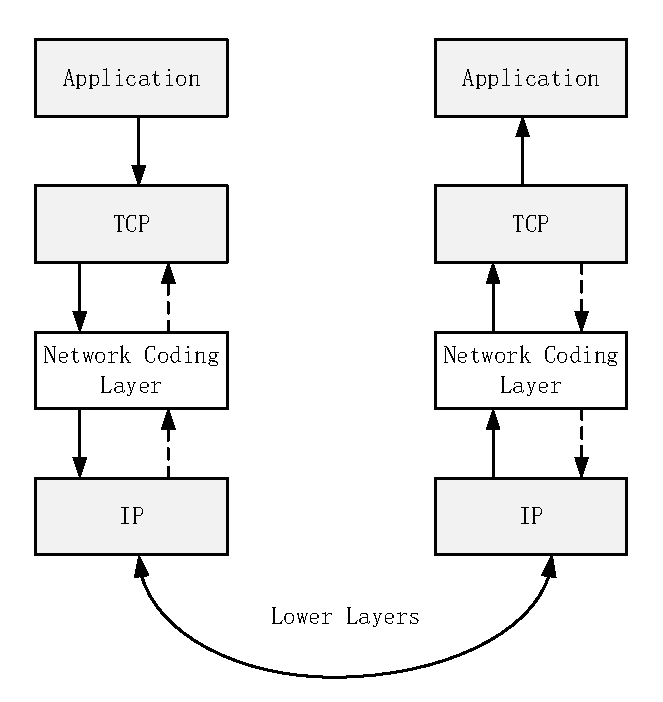
\includegraphics[height=5cm]{../figures/tcpnc.eps}
      		\caption{TCP/NC结构框图}
      		\label{fig:tcpnc}
      	\end{figure}
      	\end{column}
      \hspace{0.5em}
      \begin{column}{0.55\textwidth}
      	\footnotesize
      	\begin{block}{NC层发送端}
      		接收TCP层的数据包,
      		根据编码窗口和冗余因子对数据包进行线性组合,然后发往IP层。
      		接收端收到足够线性组合包后就可以将原始数据包解码出来。
      	\end{block}
      \begin{block}{NC层接收端}
      	接收IP层传上来的编码包,
      	满足可解条件后,
      	将原始数据宝解码出来,
      	往上传给TCP层。
      \end{block}
      \end{column}
      \end{columns}

%        \vspace{-1em}
%      其他:Tribox、Swept-sphere、 Sphere-shell、Zonotopes、圆柱形、圆锥、椭球形等等。
%      
      \note{
        上面这几个就是最常见的凸包围体。最常见的沿坐标轴方向的AABB包围盒,带方向的包围盒OBB,包围球,k面的凸包围体(k-DOP),和凸包,还有一些比较特定领域用的圆柱、圆锥形、椭球形等等。
        其中k-DOP是采用k/2对固定方向的半空间相交构成的凸包围体,是综合比较较好的包围体,因为可以通过k来调节包围体的简单性和紧致性来满足不同应用的需求。
      }
  }
\frame{
	\frametitle{Seen Packet}
	\vspace{-2em}
	\begin{myDef}[See a packet]\label{def:seepkt}
		如果一个节点根据现有的信息可以计算出如\textbf{\emph{$\left(p+q\right)$}}形式的线性组合,
		那么我们就说这个节点“\textbf{see packet \emph{$p$}}”。
		其中\textbf{$q$}本身就是只包含序号比$p$大的报文的线性组合。
		解码出某个报文也算作是“\textbf{see a packet}”,此时\textbf{$q=0$}。
	\end{myDef}
	\vspace{+1em}
	例如,接收端收到编码包$C\left[1\right]=p_1+p_2+p_3+p_4$,
	由定义\ref{def:seepkt}可知,
	接收端看到了报文$p_1$。
	如果再次接收到$C\left[2\right]=p_1+2p_2+3p_3+p_4$,
	由$C\left[2\right] - C\left[1\right] = p_2+p_3$,
	由定义\ref{def:seepkt}可知,接收端看到了报文$p_2$。
	接收端对于看到的每个报文,
	都会回复给发送端一个ACK。
	
}
   \frame{
   \frametitle{编解码示例}
     \footnotesize%%字体
     \begin{columns}[onlytextwidth]
     	\hspace{-2.0em}
     	\begin{column}{0.55\textwidth}
     		\begin{figure}
     			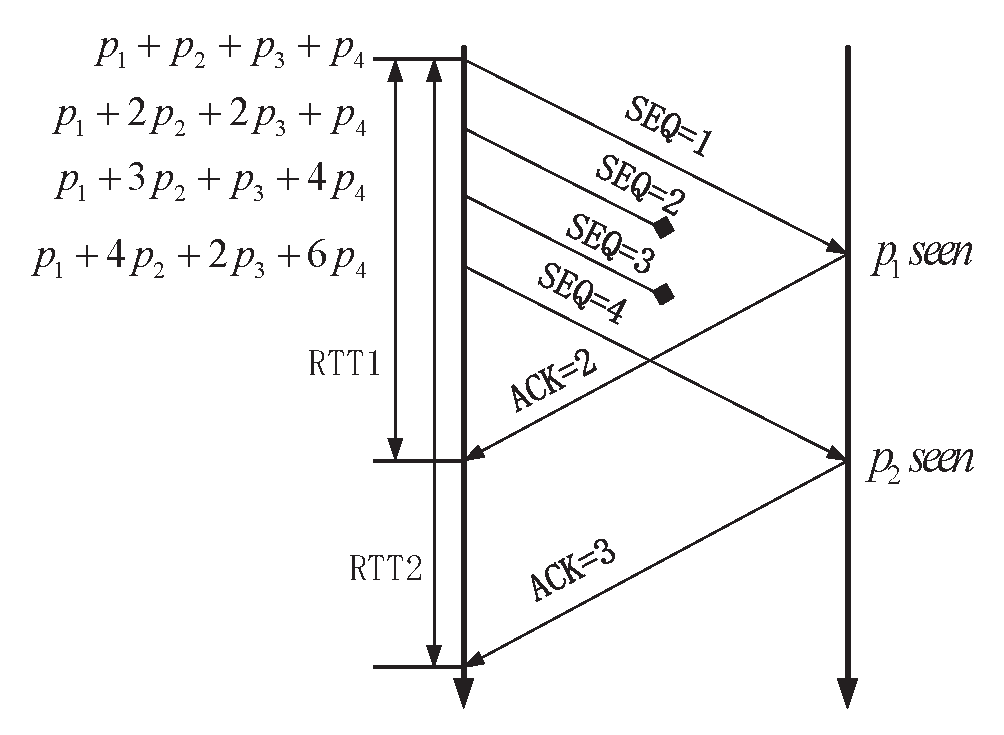
\includegraphics[height=5cm]{../figures/codingack.eps}
     			\caption{编码发送示例}
     			\label{fig:codingexp}
     		\end{figure}
     	\end{column}
     	\hspace{4.5em}

     	\begin{column}{0.40\textwidth}
     		%\footnotesize
     		% \vspace{+15em}
     		如图\ref{fig:codingexp}所示,
     		尽管$SEQ=2$和$SEQ=3$丢失,
     		但是接收端在收到$SEQ=4$的编码包后,
     		看到了报文$p_2$,
     		所以回复给发送端的是$ACK=3$。
     		对于处于接收端未解出的报文,
     		如$p_3$和$p_4$,就交给后续的冗余包来补偿。
     		
     	\end{column}
     \end{columns}
%     \textbf{$k$-DOP}\footfullcite{klosowski1998efficient}的局限性:方向\textbf{固定}且为\textbf{有限的偶数},不同模型其截面方向一致, \textbf{不够紧致};\\ 
%     而凸包很(最)紧致,但面片数量太多,构造复杂度$O(n\log n)$。
%    \begin{block}{本文凸包围体的目标}
%      \hspace{-2.0em}   \begin{minipage}{\textwidth}
%    \begin{description}
%      \item[紧致:] 能够自适应模型,根据模型形状特点有不同的方向;
%      \item[快速:] 生成凸包围体的速度要快,利用~GPU~加速;
%      \item[灵活:] 通过参数~$k$~调节凸包围体的简单性和紧致程度。
%    \end{description}
%  \end{minipage}
%    \end{block}

       \note{
       }
  }

  \subsection{TCP/NC存在问题}
   \frame{
   \frametitle{传输时延 }
    \vspace{-1em}
    \begin{myDef}[传输时延]\label{def:shiyan}
    	如果源节点产生数据报文$pkt_i$的时间为$t_{s_i}$,
    	目的节点将数据报文$pkt_i$交付给上层时间为$t_{r_i}$,
    	定义数据包的传输时延为$delay_i=t_{r_i} - t_{s_i}$。
    \end{myDef}
   \begin{block}{解码导致的时延}
   	TCP/NC的基本思想是利用发送端的编码将链路的丢包问题后延,
   	当发送端的冗余包足够弥补链路丢包后,
   	丢包就被掩盖。
   	带来的问题是数据包的传输时延变大。
   	以图\ref{fig:codingexp}为例,
   	如果补偿$SEQ=2$的冗余包为$SEQ=7$,
   	那么$p_2$需要等到$SEQ=7$才能被接收端的NC层交付给上层TCP。
   	那么$p_2$的传输时延为$delay_2 = t_{r_7} - t_{s_2}$。
   	   \end{block}

%   \begin{block}{分类}
%     \begin{description}
%       \item[加速结构:] SPT(如四叉树、KD~树等)~v.s~\textbf{BVH}(OBB树、$k$-DOP树等)
%       \item[表现形式:] \textbf{刚体}~v.s~可变形,凸体~v.s~凹体,CSG~v.s~参数曲面~v.s~\textbf{多边形网格}
%       \item[碰撞环境:] \textbf{成对}~v.s~\textbf{多体},\textbf{静止}~v.s~\textbf{运动},\textbf{离散}~v.s~连续
%     \end{description}
%   \end{block}
   
   \note{
    (介绍PPT后),本文后面的实验就是基于BVH的,不可变形的三角网格。//现在研究较多的是连续的可变形的碰撞检测布料模拟头发模拟等。
   }
  }
%
%  \frame{
%    \frametitle{基于~BVH~的碰撞检测算法}
%    \begin{columns}[onlytextwidth]
%      \begin{column}{0.35\textwidth}
%        \vspace{-1.5em}
%        \begin{figure}[htbp]
%            \begin{center}
%            \begin{boxedminipage}{1\textwidth}
%            \subfloat{\label{lbl:bvh-bunny-center-0.png}}
%              {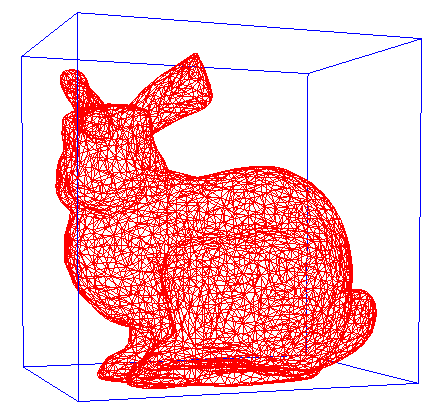
\includegraphics[height=1.4cm]{bvh-bunny-center-0.png}}
%            \subfloat{\label{lbl:bvh-bunny-center-1.png}}
%              {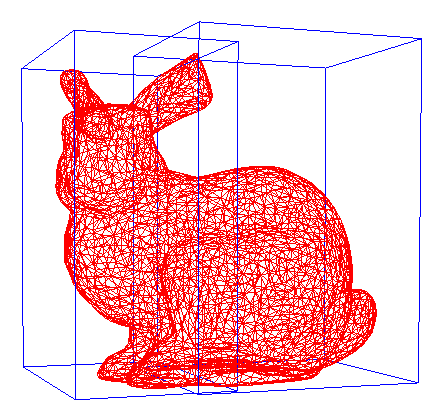
\includegraphics[height=1.4cm]{bvh-bunny-center-1.png}}
%            \\
%            \subfloat{\label{lbl:bvh-bunny-center-2.png}}
%              {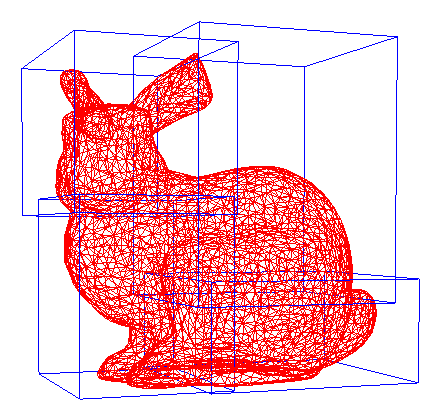
\includegraphics[height=1.4cm]{bvh-bunny-center-2.png}}
%            \subfloat{\label{lbl:bvh-bunny-center-3.png}}
%              {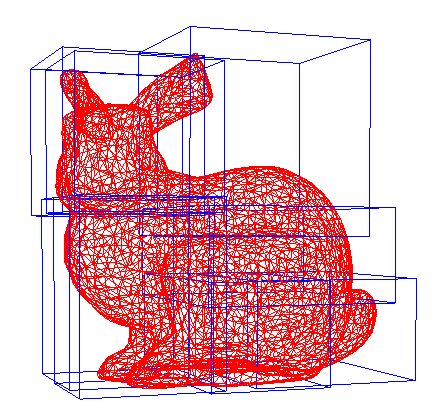
\includegraphics[height=1.4cm]{bvh-bunny-center-3.png}}
%            \\\hspace{0.5cm}
%            \subfloat{\label{lbl:bvh-bunny-center-4.png}}
%              {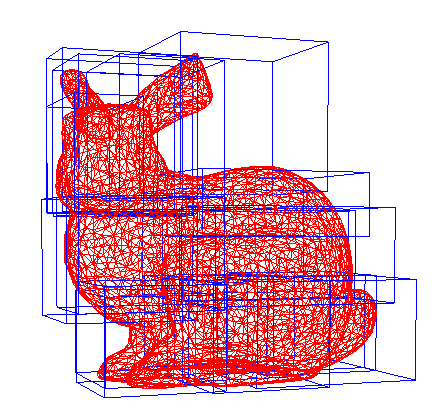
\includegraphics[height=1.5cm]{bvh-bunny-center-4.png}}
%            \subfloat{\label{lbl:bvh-bunny-center-5.png}}
%              {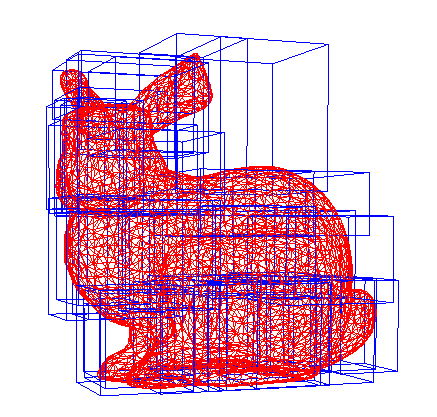
\includegraphics[height=1.5cm]{bvh-bunny-center-5.png}}
%            \\
%            \subfloat{\label{lbl:bvh-bunny-center-6.png}}
%              {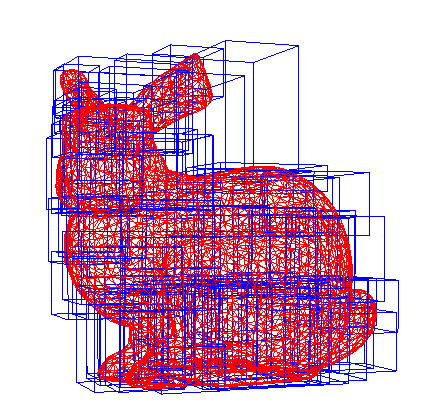
\includegraphics[height=1.5cm]{bvh-bunny-center-6.png}}
%            \subfloat{\label{lbl:bvh-bunny-center-7.png}}
%              {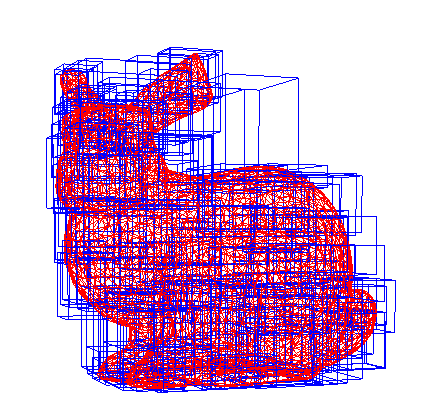
\includegraphics[height=1.5cm]{bvh-bunny-center-7.png}}
%            \end{boxedminipage}
%            \vspace{-0.5em}
%          \caption{八层~BVH~示例}
%          \label{lbl:bvh-example}
%          \end{center}
%          \end{figure}
%      \end{column}
%      \hspace{0.5em}
%      \begin{column}{1.2\textwidth}
%      \vspace{0.2em}
%         \scalebox{0.5}{
%              \begin{minipage}{1.0\textwidth}
%      \vspace{-2em}
%           \begin{algorithm}[H]
%              \caption{自顶向下层次遍历~BVH~}
%              \label{alg:traverse-bvh-tree}
%              \begin{algorithmic}[1]
%              \Require
%              两个~BVH~树的根节点~$node_1$,$node_2$
%              \Ensure
%              模型是否相交
%              \Function {TraverseBVHTree}{$node_1, node_2$}
%                \If{$node_1.bv \cap node_2.bv = \emptyset$}
%                  \State \Return{\textbf{False}}
%                  \Comment{包围体重合测试, 包围体不相交直接返回}
%                \Else
%                    \If {$node_1.children = \emptyset$}
%                         \If {$node_2.children = \emptyset$}
%                         \State \Comment{最底层叶子节点原生几何相交测试}
%                         \State \Return {\Call{CheckIntersection}{$node_1.primitives, node_2.primitives$}}
%                         \Else
%                            \ForAll {$child \in node_2.children$}
%                            \State \Call{TraverseBVHTree}{$node_1, child$} \Comment{递归调用}
%                            \EndFor
%                         \EndIf
%                    \Else
%                         \ForAll {$child \in node_1.children$}
%                         \State \Call{TraverseBVHTree}{$child, node_2$}  \Comment{递归调用}
%                         \EndFor
%                    \EndIf
%                \EndIf
%              \EndFunction
%              \end{algorithmic}
%              \end{algorithm}
%              \end{minipage}
%            }
%      \\
%      \scriptsize \hspace{1em}代价函数: $T_{cost} = n_v * C_v + n_p * C_p + (n_u * C_u)$(运动)
%      \end{column}
%    \end{columns}
%    \note{
%      基于包围体树的碰撞检测算法, 一般首先都会初始化环境然后构建层次结构的包围体树,碰撞检测时从顶层开始逐渐往下层遍历,到最底层叶子节点后开始三角网格模型相交测试,
%      当发现三角网格相交后立即终止遍历,确定模型发生碰撞。
%      评价碰撞检测算法的指标一般用上面这个公式来衡量,其中nv和 np分别表示参与包围体节点相交测试的数量和参与原始几何相交测试的数量,Cv和 Cp则表示相应的平均测试耗费的代价。
%      当在运动场景时还需要加上nu和 Cn就是模型旋转或者运动后包围体更新的数量和更新的代价。
%      本文算法就是尽早发现包围体不相交的情况,减少np和cp的数量。
%    }
%}

\section{网络编码与TCP/NC协议}

%%==========第一节==========
\subsection{网络编码理论基础}
%%网络编码概念
\begin{frame}[allowframebreaks,t]
	\frametitle{网络编码概念}
	\begin{block}{网络编码}
		\footnotesize
		在包交换网络中,
		中间节点不仅仅是简单地路由转发接收到的数据包,
		而是对它们进行一些函数操作并计算、转发操作结果\footfullcite{Ahlswede2000}。
	\end{block}
	\vspace{-1em}
	\begin{figure}[t]
	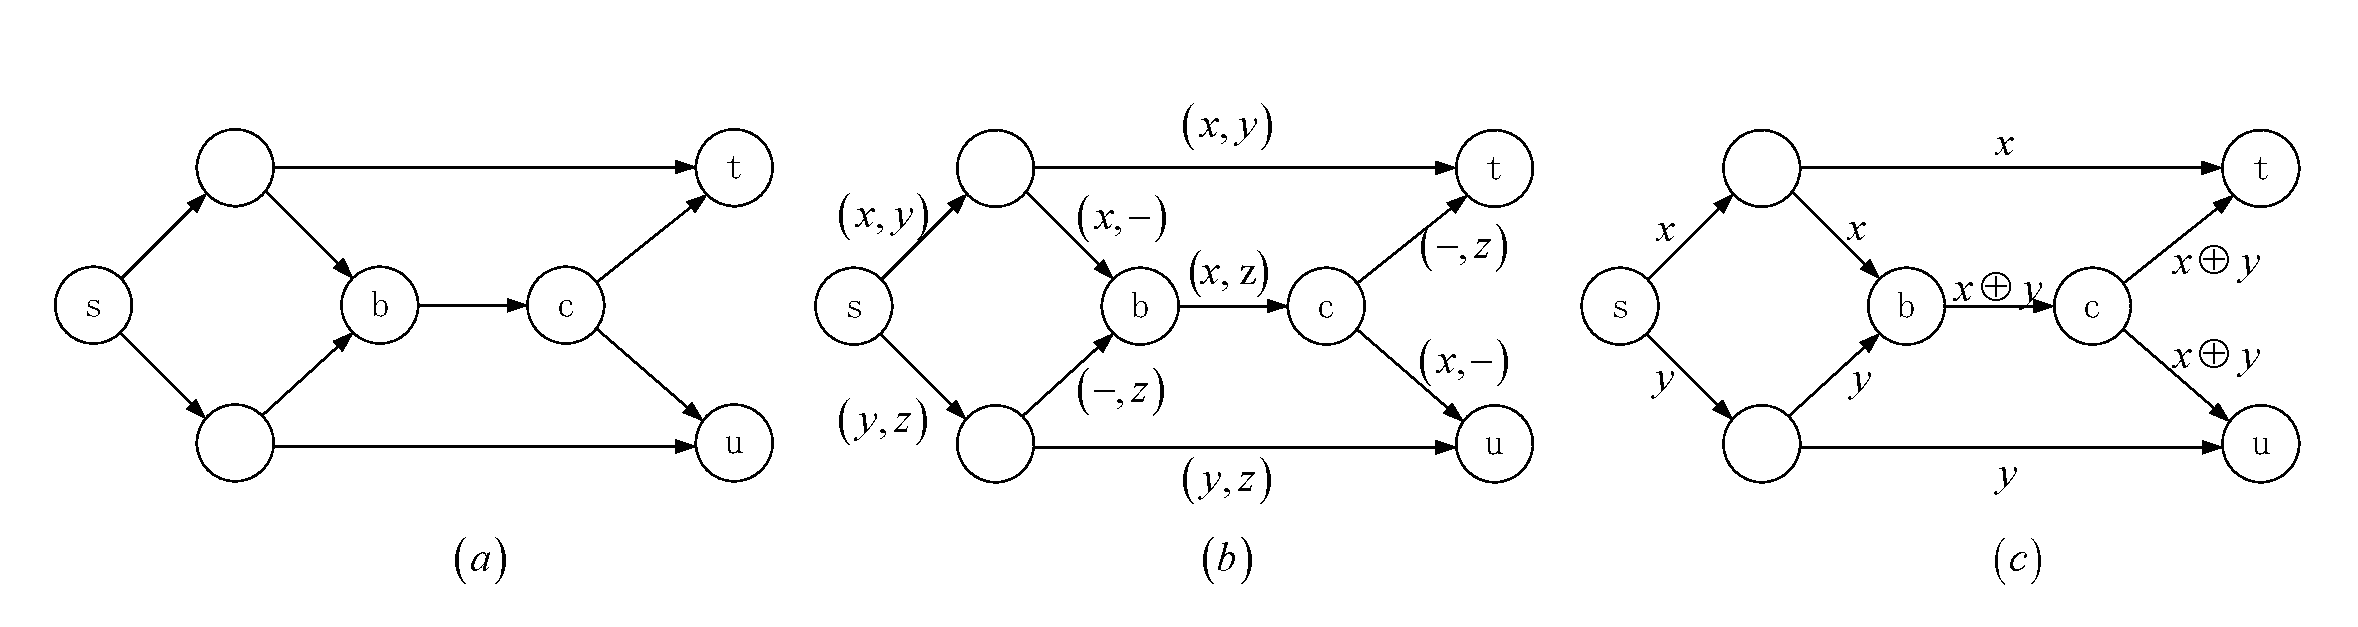
\includegraphics[height=3.5cm]{../figures/butter.eps}
	\caption{蝶形网络}
	\label{fig:butter}
	\end{figure}
	图\ref{fig:butter}(b)为传统的路由算法,
	其多播吞吐量为1.5。
	图\ref{fig:butter}(c)为应用了网络编码的路由算法,
	其多播吞吐量为2,且是理论上最大的网络多播吞吐量。
	\begin{mytheorem}
	一个网络的最大多播吞吐量取决于分割源节点和目的节点的最小割集\supercite{Ahlswede2000}。
	\end{mytheorem}
	\note{
		运用网络编码可以提高网络吞吐率、均衡网络负载和提高网络带宽利用率。
	}
\end{frame}
%%网络编码的一个简单例子
%\begin{frame}[t]
%	\frametitle{网络编码的一个简单例子}
%	\vspace{-1.5em}
%	\begin{figure}[t]
%		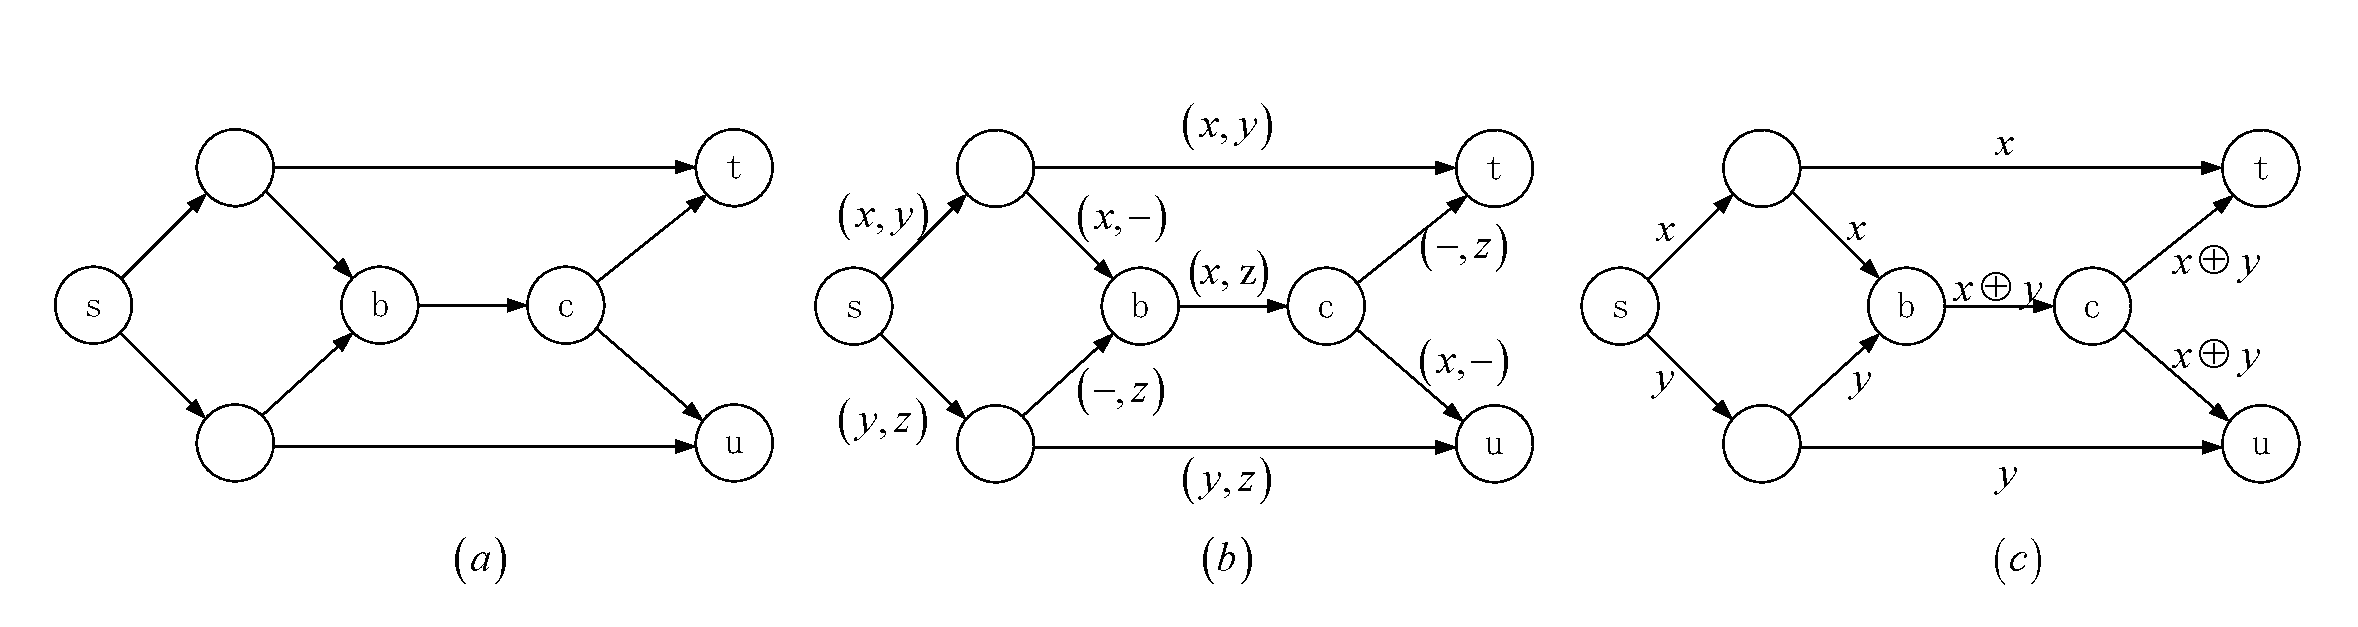
\includegraphics[height=2.5cm]{../figures/butter.eps}
%		\caption{蝶形网络}
%		\label{fig:butter}
%	\end{figure}
%	\vspace{-1em}
%%	图\ref{fig:butter}为一个包交换模型。
%	图\ref{fig:butter}(b)为传统的路由算法,
%	其多播吞吐量为1.5。
%	图\ref{fig:butter}(c)为应用了网络编码的路由算法,
%	其多播吞吐量为2,且是理论上最大的网络多播吞吐量。
%	\begin{mytheorem}
%	一个网络的最大多播吞吐量取决于分割源节点和目的节点的最小割集\supercite{Ahlswede2000}。
%	\end{mytheorem}
%
%\end{frame}
%%线性网络编码
\begin{frame}[t,allowframebreaks]
	\frametitle{线性网络编码}
	%%第一帧
	令$\left(p_1,p_2,\dots,p_r\right)^{T}$表示进入源节点$s$的数据包${{\rm X}_{{\rm I}\left( s \right)}}$。
	每个数据包$p_i$都是$\mathbb{F}_{q}$上长度为$m$的矢量。
	我们可以用一个定义在$\mathbb{F}_{q}$上的$r \times m$矩阵来表示${\rm X}_{{\rm I}\left( s \right)}$,
	该矩阵的第$i$行是$p_{i}$。
	\\
	\vspace{1em}
	本地编码函数是$\mathbb{F}_{q}$上的线性函数,即任意中间节点$v$输出的数据包列向量${\rm X}_{{\rm O}\left( v \right)}$与其接收到的数据包列向量${\rm X}_{{\rm I}\left( v \right)}$之间的关系可以用以下线性方程组表示:
	\begin{equation}\label{eq:xianxingfangchengzu}
	{\rm X}_{{\rm O}\left( v \right)}={\rm L}_{v}{\rm X}_{{\rm I}_{\left( v \right)}}
	\end{equation}
	其中,${\rm L}_{v}$是定义在${\mathbb{F}}_{q}$上的系数矩阵。
	考虑到网络中只允许线性操作,
	因此任意边上传输的数据包都是原数据包$p_{1},p_{2},\dots,p_{r}$的线性组合。
	\newpage
	%%第二帧
	也就是$\forall v \in V$,有
	\begin{equation}\label{eq:xishujuzheng}
	{\rm X}_{{\rm I}\left( v \right)}=G_{v}\left[ {\begin{array}{*{20}{c}}
		{{p_1}}\\
		\vdots \\
		{{p_r}}
		\end{array}} \right]
	\end{equation}
	\begin{columns}[onlytextwidth]
		\vspace{3em}
		\begin{column}{0.6\textwidth}
			其中,$G_{v}$是定义在$\mathbb{F}_{q}$上的系数矩阵,
			也称为$v$的全局转移矩阵。
			${\rm G}_{v}$的每一行都对应一条边$e \in {\rm I}_{\left( v \right)}$,
			称为边$e$的全局编码向量。
			图\ref{fig:zhuanyi}为标示了本地转移矩阵的蝶形网络,
			我们可以得到在目的节点$t$和$u$的全局转移矩阵为:
		\end{column}
		\begin{column}{0.4\textwidth}
			\vspace{-1.5em}
			\begin{figure}
				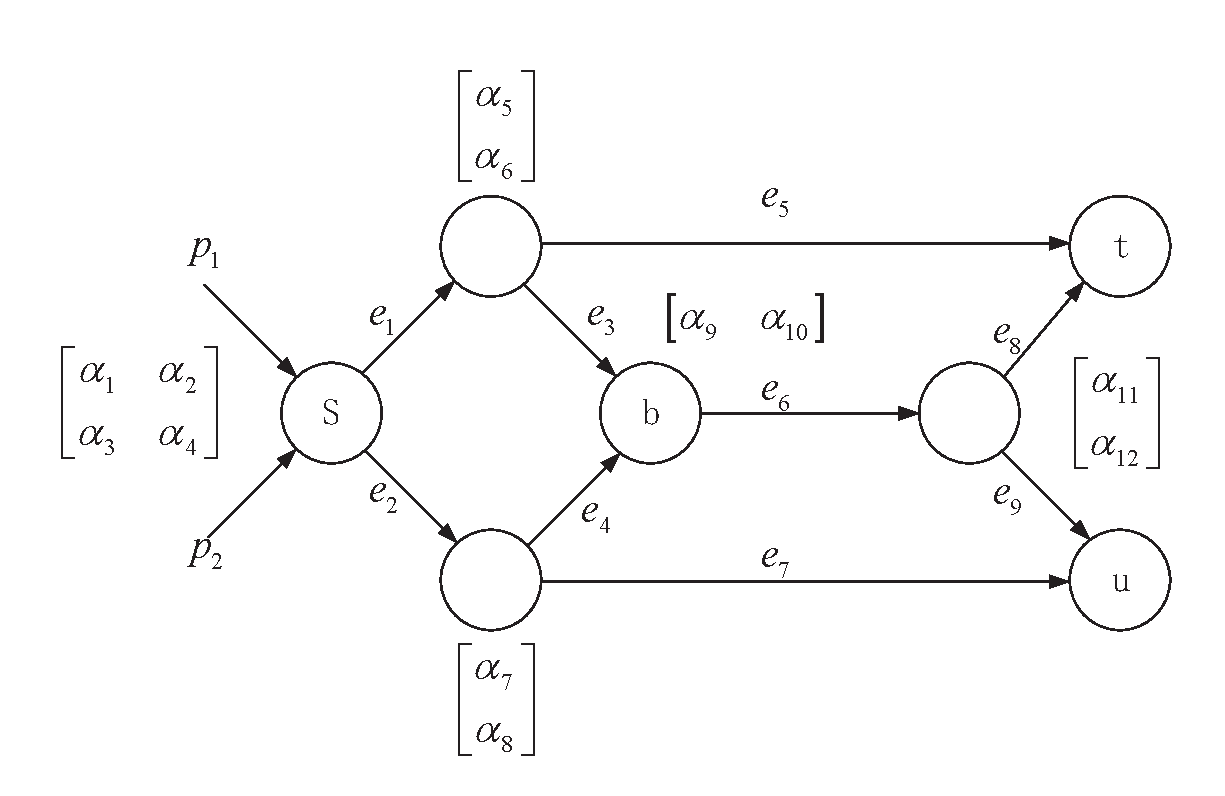
\includegraphics[height=3cm]{../figures/zhuanyi.eps}
				\caption{标注了转移矩阵的蝶形网络}
				\label{fig:zhuanyi}
			\end{figure}
		\end{column}
	\end{columns}
	
	\newpage
	\begin{eqnarray}\label{eq:quanjuzhuanyi}
	{G_t} = \left[ {\begin{array}{*{20}{c}}
		{{\alpha _1}{\alpha _5}}&{{\alpha _2}{\alpha _5}}\\
		{{\alpha _1}{\alpha _6}{\alpha _9}{\alpha _{11} }+{\alpha _3}{\alpha _7}{\alpha _{10}}{\alpha _{11} }}&{{\alpha _2}{\alpha _6}{\alpha _9}{\alpha _{11}}+{\alpha _4}{\alpha _7}{\alpha _{10}}{\alpha _{11}}}
		\end{array}} \right] \nonumber \\
	{G_u}= \left[ {\begin{array}{*{20}{c}}
		{{\alpha _1}{\alpha _6}{\alpha _9}{\alpha _{12} }+{\alpha _3}{\alpha _7}{\alpha _{10}}{\alpha _{12} }}&{{\alpha _2}{\alpha _6}{\alpha _9}{\alpha _{12}}+{\alpha _4}{\alpha _7}{\alpha _{10}}{\alpha _{12}}}\\
		{{\alpha _3}{\alpha _8}}&{{\alpha _4}{\alpha _8}}
		\end{array}} \right]
	\end{eqnarray}
	对于目的节点$t$来说,
	当且仅当$\left|{\rm I}\left(t\right)\right| \times r$阶全局转移矩阵$G_{t}$的秩为$r$时,
	$t$才能恢复出$\left(p_1,p_2,\dots,p_r\right)$中的所有元素。
	因为只有$G_t$满秩时,
	才存在满足${G_t}^{-1}G_t={\rm I}_r$的左逆矩阵,
	其中${\rm I}_r$是$r \times r$阶单位矩阵。
	只需$G_{t}$满秩,
	而不要求$G_{t}$是可求逆的方阵。
	目的节点$t$可以通过计算${G_t}^{-1}{\rm X}_{{\rm I}\left(t\right)}$得到$\left(p_1,p_2,\dots,p_r\right)^{T}$。

	\note{
		换句话说,$v$输出的每个数据包( ${\rm X}_{{\rm O}\left( v \right)}$的一个分量)都可以看做是进入$v$的多个数据包在$\mathbb{F}_{q}$上的线性组合。
	}
\end{frame}
%%两种网络编码
\begin{frame}[t,allowframebreaks]
	\frametitle{Batch Coding和Pipeline Coding}
	将网络编码应用于提升有损链路的吞吐率,
	其应用方式主要有两种:Batch Coding和Pipeline Coding。
	\begin{block}{Batch Coding}
		\footnotesize
		定义\emph{generation}为数据包的集合,作为编解码的整体。
		源节点和网络中的中间节点在同一个\emph{generation}上进行编码,
		目的节点只有在收到足够多的编码报文后,
		才能一次性解出这一个\emph{generation}中的所有原始报文。
	\end{block}
	假设$p_1,p_2,\dots$为原始数据包,\emph{k}为\emph{generation}的大小,
	第$i^{th}$个\emph{generation}产生的一个编码包可以被表示为:
	\begin{equation}\label{eq:batch-pkt}
	c = \sum\limits_{j = 1}^k {{e_j}{p_{i \times k + j}}}
	\end{equation}
	\newpage
	\begin{block}{Pipeline Coding}
		\footnotesize
		无需等待一个\emph{generation}满秩,
		每当一个数据报文来之后,
		就会产生一个编码包。
		目的节点会逐步解出原始报文。
	\end{block}
	Pipeline Coding的编码函数为:
	\begin{equation}\label{eq:pipelinecoding}
	c = \sum\limits_{j = 1}^m {{e_j}{p_{i \times k + j}}}
	\end{equation}
	其中\emph{m}表示目前在编码缓存中数据包的个数。
	图\ref{fig:codingMechanism}为两种编码方式示例,
	其中冗余度都为1.25,即每发送4个报文发送一个冗余包。
	\newpage
	 \begin{figure}
		\centering
		\begin{boxedminipage}{1\textwidth}
		\subfloat[]{
			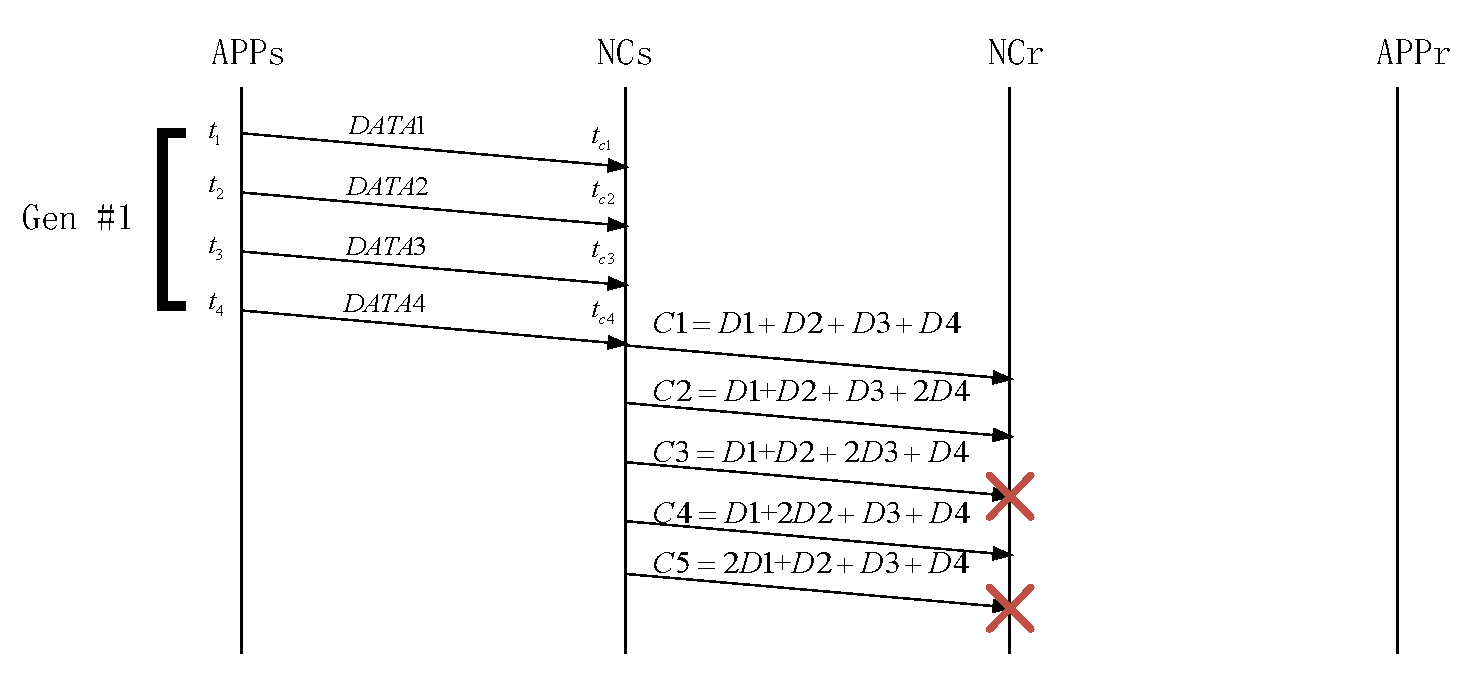
\includegraphics[width=2.5in]{../figures/batchundecode.eps}
			\label{fig:batchcoding}
		}
		\subfloat[]{
			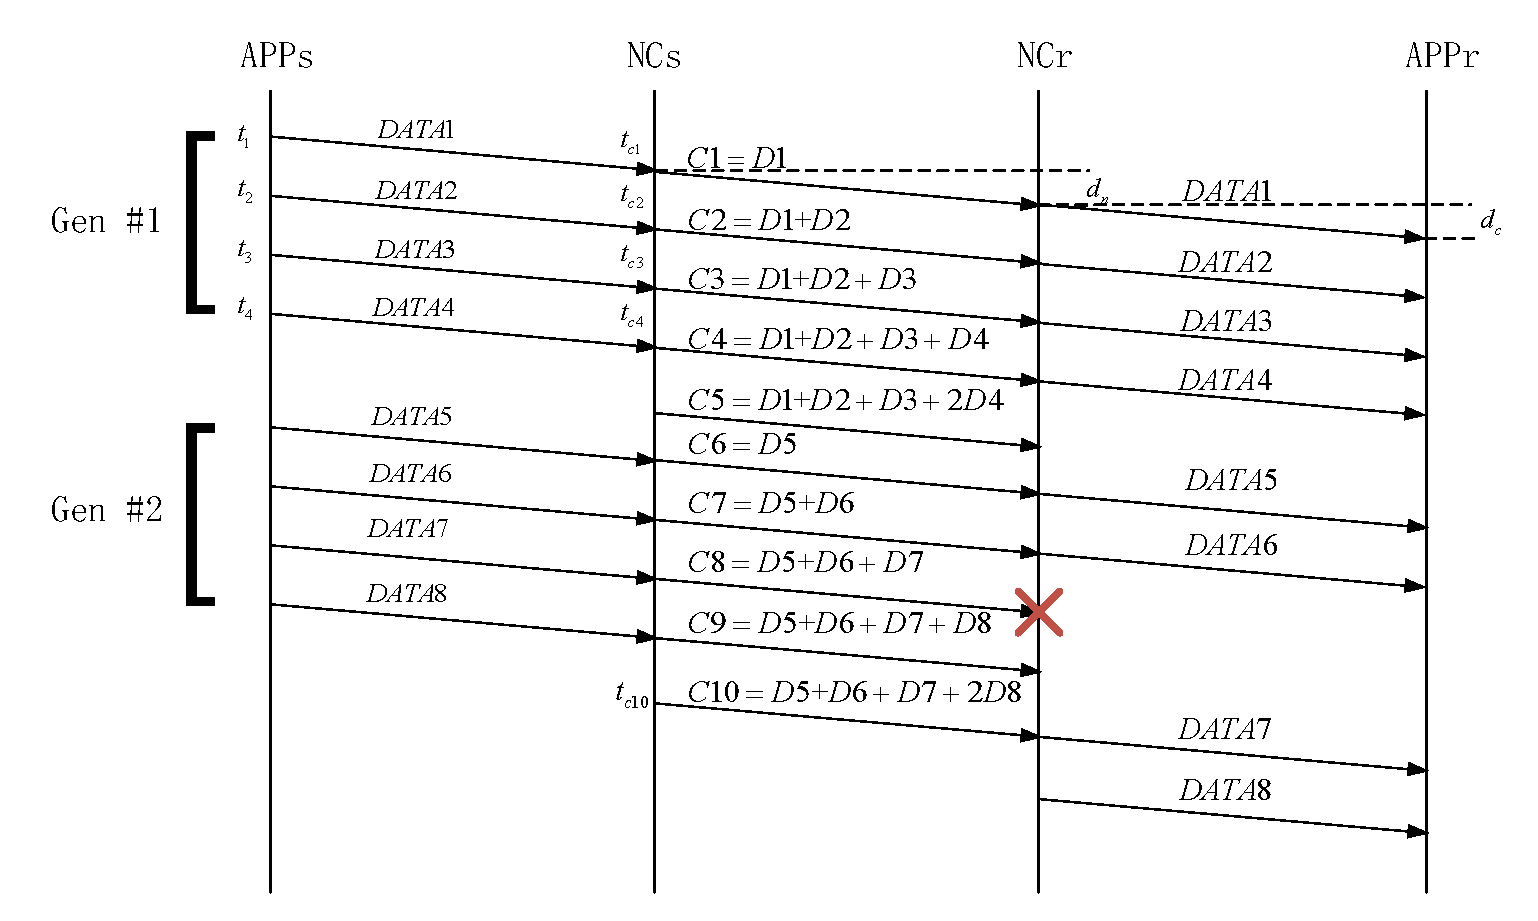
\includegraphics[width=2.5in]{../figures/pipeline.eps}
			\label{fig:pipelinecoding}
		}
		\end{boxedminipage}
		\caption{\small (a) Batch Coding ~~ (b) Pipeline Coding}
		\label{fig:codingMechanism}
	\end{figure}
	\vspace{-1em}
	采用Pipeline Coding的优点:解码时延更低。
	\note{
		由于每个编码数据包都是同一个\emph{generation}的数据包的线性组合,
		在源节点就引入了一个延时。
		换句话说,
		同一个\emph{generation}里面前面的报文需要等后面的报文,
		直到这个\emph{generation}满秩候,才可进行编码。
		在目的节点处,
		同一个\emph{generation}的报文,
		要么都解码,
		要么一个都解不出。
		i表示第i个\emph{generation}。
	}
\end{frame}

%%==========第二节==========
\subsection{TCP/NC协议}
%%ACK On degree of freedom
\begin{frame}[t,allowframebreaks]
	\frametitle{ACK On degree of freedom}
	TCP、ARQ协议中的ACK都是对原始数据包的确认,
	\emph{ACK On degree of freedom}\footfullcite{4595268}则对\emph{自由度}进行确认。
	\begin{myDef}[See a packet]\label{def:seepkt}
	如果一个节点根据现有的信息可以计算出如\textbf{\emph{$\left(p+q\right)$}}形式的线性组合,
	那么我们就说这个节点“\textbf{see packet \emph{$p$}}”。
	其中\textbf{$q$}本身就是只包含序号比$p$大的报文的线性组合。
	解码出某个报文也算作是“\textbf{see a packet}”,此时\textbf{$q=0$}。
	\end{myDef}
	接收端如果\emph{see packet p},那么就需要对\emph{p}进行ACK。
	表\ref{tab:ack-on-degree-of-freedom}为\emph{ACK on degree of freedom}的例子。
	\newpage
	\vspace*{-3em}
	\begin{table}  
	\centering  
	\fontsize{6.5}{8}\selectfont  
	\begin{threeparttable}  
		\caption{\emph{ACK on degree of freedom} 例子}  
		\label{tab:ack-on-degree-of-freedom}  
		\begin{tabular}{c|c|c|c|c|c}  
			\toprule  
			\multirow{2}{*}{Time} &\multirow{2}{*}{Sender's queue} & \multirow{2}{*}{Transmitted packet} & \multirow{2}{*}{Channel state}&  
			\multicolumn{2}{c}{ Destination Node \emph{A}}\cr  
			\cmidrule(lr){5-6}  
			\hspace{1cm}&\hspace{1cm}&\hspace{1cm}&\hspace{1cm}&Decoded&Seen but not decoded\cr  
			\midrule  
			1&$p_{1}$&$p_{1}$&$\nrightarrow A$&\hspace{1cm}&\hspace{1cm}\cr
			\hline  
			2&$p_{1}$,$p_{2}$&$p_{1} \oplus p_{2}$&$\rightarrow A$&\hspace{1cm}&$p_{1}$\cr 
			\hline 
			3&$p_{2}$,$p_{3}$&$p_{2} \oplus p_{3}$&$\rightarrow A$&\hspace{1cm}&$p_{1}$,$p_{2}$\cr
			\hline  
			4&$p_{3}$,$p_{4}$&$p_{3} \oplus p_{4}$&$\nrightarrow A$&\hspace{1cm}&$p_{1}$,$p_{2}$\cr
			\hline  
			5&$p_{3}$,$p_{4}$,$p_{5}$&$p_{3} \oplus p_{4} \oplus p_{5}$&$\rightarrow A$&\hspace{1cm}&$p_{1}$,$p_{2}$,$p_{3}$\cr
			\hline  
			6&$p_{4}$&$p_{4}$&$\rightarrow A$&$p_{4}$&$p_{1}$,$p_{2}$,$p_{3}$,$p_{5}$\cr
			\hline
			7&$p_{5}$&$p_{5}$&$\rightarrow A$&$p_{1}$,$p_{2}$,$p_{3}$,$p_{4}$,$p_{5}$&\hspace{1cm}\cr    
			\bottomrule  
		\end{tabular}  
	\end{threeparttable}  
	\end{table}
	优点:发送端可以减小发送队列的长度。
\end{frame}

\begin{frame}[t]
	\frametitle{TCP/NC概述}
	为了提高标准TCP在有损信道环境下的性能,
	Sundararajan等人提出了TCP/NC。
	将网络编码和TCP结合起来,
	在发送端冗余编码,
	掩盖链路中出现的丢包。
	\\
	其关键点有:
	\begin{block}{TCP/NC关键点}
		\begin{enumerate}
			\item 在发送端的TCP层和IP层插入一个网络编码层,
			在编码层对数据包进行线性网络编码。
			\item 利用\emph{ACK On degree of freedom}的概念,
			重新定义TCP中ACK的概念。
			\item 发送端通过冗余编码来补偿链路中出现的丢包
		\end{enumerate}
	\end{block}
\end{frame}

%%TCP/NC框图
\frame{
	\frametitle{TCP/NC框图}
	\begin{columns}[onlytextwidth]
		\hspace{-4em}
		\begin{column}{0.45\textwidth}
			\vspace{-1em}
			\begin{figure}
      			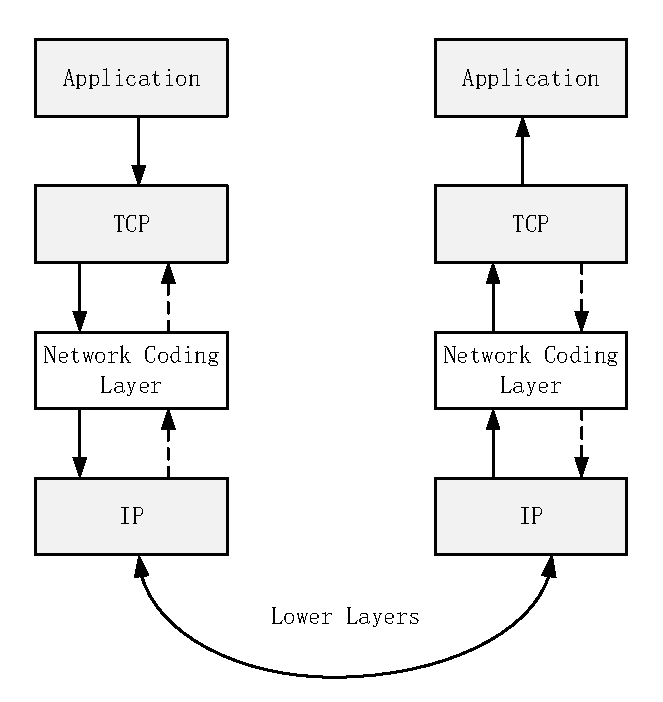
\includegraphics[height=5cm]{../figures/tcpnc.eps}
      			\caption{TCP/NC结构框图}
      			\label{fig:tcpnc}
    		\end{figure}
      	\end{column}
      	\begin{column}{0.65\textwidth}
      		\footnotesize
      		\begin{block}{NC层发送端}
      			\begin{enumerate}
      				\item 接收TCP层的数据包,
      				根据编码窗口和冗余因子对数据包进行线性组合,
      				然后发往IP层。
      				\item 处理接收端回复的ACK报文,
      				并据此删除编码队列的报文。
      			\end{enumerate}
      		\end{block}
      		\begin{block}{NC层接收端}
      			\begin{enumerate}
      				\item 接收IP层传上来的编码包,
      				并进行解码运算。
      				如果有新的报文被看到,
      				回复发送端ACK报文;
      				如果有新的原始数据包被解码,
      				将其传给上层TCP。
      				\item 拦截上层TCP下来的ACK报文。
      			\end{enumerate}
      		\end{block}
      \end{column}
  \end{columns}
  \note{
  }
}

%\frame{
%	\frametitle{Seen Packet}
%	\vspace{-2em}
%	\begin{myDef}[See a packet]\label{def:seepkt}
%		如果一个节点根据现有的信息可以计算出如\textbf{\emph{$\left(p+q\right)$}}形式的线性组合,
%		那么我们就说这个节点“\textbf{see packet \emph{$p$}}”。
%		其中\textbf{$q$}本身就是只包含序号比$p$大的报文的线性组合。
%		解码出某个报文也算作是“\textbf{see a packet}”,此时\textbf{$q=0$}。
%	\end{myDef}
%	\vspace{+1em}
%	例如,接收端收到编码包$C\left[1\right]=p_1+p_2+p_3+p_4$,
%	由定义\ref{def:seepkt}可知,
%	接收端看到了报文$p_1$。
%	如果再次接收到$C\left[2\right]=p_1+2p_2+3p_3+p_4$,
%	由$C\left[2\right] - C\left[1\right] = p_2+p_3$,
%	由定义\ref{def:seepkt}可知,接收端看到了报文$p_2$。
%	接收端对于看到的每个报文,
%	都会回复给发送端一个ACK。
%	
%}
%%编解码示例
\begin{frame}[t]
	\frametitle{编解码示例}
 	\begin{columns}[t,onlytextwidth]
    	\hspace{-2.0em}
    	\begin{column}{0.55\textwidth}
    		\vspace{-2em}
    		\begin{figure}
    			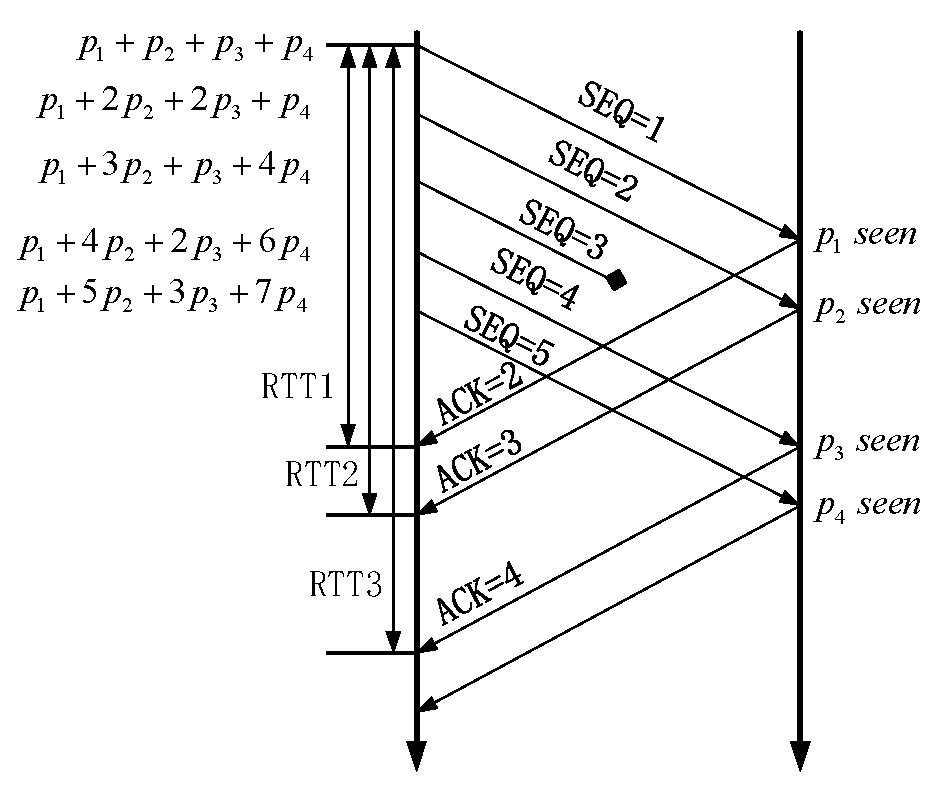
\includegraphics[height=5cm]{figures/encodingexp.eps}
    			\caption{编码发送示例}
    			\label{fig:codingexp}
    		\end{figure}
    	\end{column}
    	\hspace{2.5em}
    	\begin{column}{0.45\textwidth}
    		图\ref{fig:codingexp}所示为冗余度1.25时编码发送的一个示例。\\
    		\vspace{1em}
    		尽管$SEQ=3$丢失,
    		但是接收端在收到$SEQ=4$的编码包后,
    		看到了报文$p_3$,
    		所以回复给发送端的是$ACK=4$。
    		在收到冗余报文$SEQ=5$后,
    		看到了$p_4$,
    		同时也将$p_1 \sim p_4$全部解出。\\
    		\vspace{1em}
    		链路的丢包在发送端的TCP层看来仅仅是RTT的增大。
    	\end{column}
	\end{columns}
\end{frame}

\begin{frame}
	\frametitle{冗余度}
	TCP/NC能够抵抗链路丢包的关键是发送端进行了冗余编码。
	冗余度决定了TCP/NC发送冗余包的多少。
	\\
	理论上,当链路的丢包率为$\rho$时,设置的冗余度\emph{R}应该为
	\begin{equation}\label{eq:redundancy}
	R=\dfrac{1}{1 - \rho}
	\end{equation}
	此时,链路中出现的丢包刚好全部被冗余包补偿。
\end{frame}


%\frame{
%\frametitle{传输时延 }
%\vspace{-1em}
%\begin{myDef}[传输时延]\label{def:shiyan}
%   	如果源节点产生数据报文$pkt_i$的时间为$t_{s_i}$,
%   	目的节点将数据报文$pkt_i$交付给上层时间为$t_{r_i}$,
%   	定义数据包的传输时延为$delay_i=t_{r_i} - t_{s_i}$。
%\end{myDef}
%\begin{block}{解码导致的时延}
%  	TCP/NC的基本思想是利用发送端的编码将链路的丢包问题后延,
%  	当发送端的冗余包足够弥补链路丢包后,
%  	丢包就被掩盖。
%  	带来的问题是数据包的传输时延变大。
%  	以图\ref{fig:codingexp}为例,
%  	如果补偿$SEQ=2$的冗余包为$SEQ=7$,
%  	那么$p_2$需要等到$SEQ=7$才能被接收端的NC层交付给上层TCP。
%  	那么$p_2$的传输时延为$delay_2 = t_{r_7} - t_{s_2}$。
%   \end{block}
%
%\note{
%(介绍PPT后),本文后面的实验就是基于BVH的,不可变形的三角网格。//现在研究较多的是连续的可变形的碰撞检测布料模拟头发模拟等。
%}
%}
%
%  \frame{
%    \frametitle{基于~BVH~的碰撞检测算法}
%    \begin{columns}[onlytextwidth]
%      \begin{column}{0.35\textwidth}
%        \vspace{-1.5em}
%        \begin{figure}[htbp]
%            \begin{center}
%            \begin{boxedminipage}{1\textwidth}
%            \subfloat{\label{lbl:bvh-bunny-center-0.png}}
%              {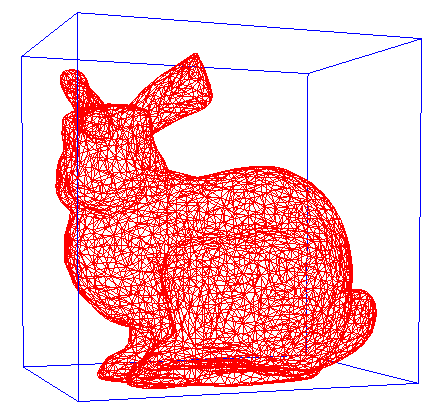
\includegraphics[height=1.4cm]{bvh-bunny-center-0.png}}
%            \subfloat{\label{lbl:bvh-bunny-center-1.png}}
%              {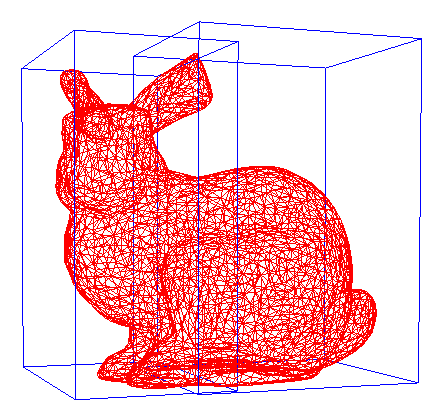
\includegraphics[height=1.4cm]{bvh-bunny-center-1.png}}
%            \\
%            \subfloat{\label{lbl:bvh-bunny-center-2.png}}
%              {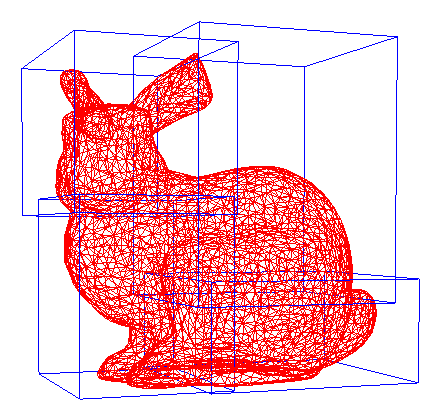
\includegraphics[height=1.4cm]{bvh-bunny-center-2.png}}
%            \subfloat{\label{lbl:bvh-bunny-center-3.png}}
%              {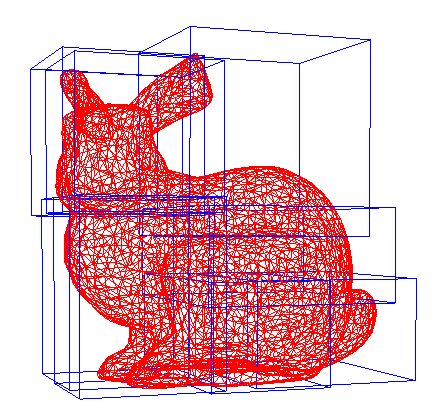
\includegraphics[height=1.4cm]{bvh-bunny-center-3.png}}
%            \\\hspace{0.5cm}
%            \subfloat{\label{lbl:bvh-bunny-center-4.png}}
%              {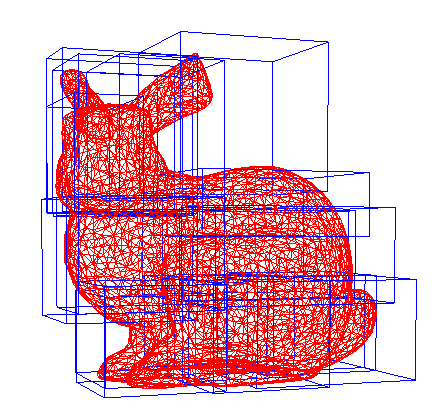
\includegraphics[height=1.5cm]{bvh-bunny-center-4.png}}
%            \subfloat{\label{lbl:bvh-bunny-center-5.png}}
%              {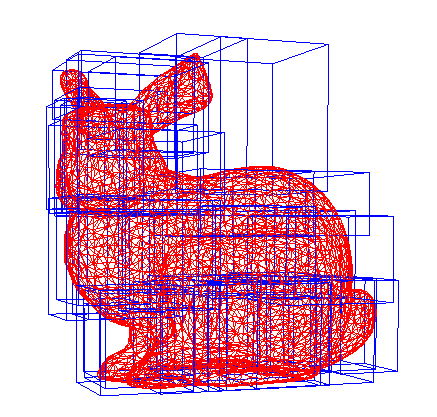
\includegraphics[height=1.5cm]{bvh-bunny-center-5.png}}
%            \\
%            \subfloat{\label{lbl:bvh-bunny-center-6.png}}
%              {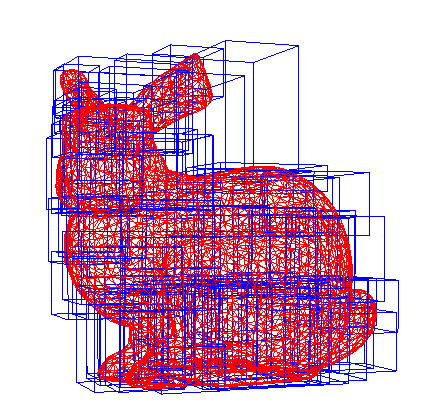
\includegraphics[height=1.5cm]{bvh-bunny-center-6.png}}
%            \subfloat{\label{lbl:bvh-bunny-center-7.png}}
%              {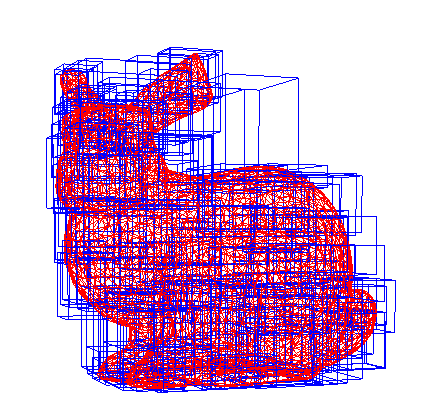
\includegraphics[height=1.5cm]{bvh-bunny-center-7.png}}
%            \end{boxedminipage}
%            \vspace{-0.5em}
%          \caption{八层~BVH~示例}
%          \label{lbl:bvh-example}
%          \end{center}
%          \end{figure}
%      \end{column}
%      \hspace{0.5em}
%      \begin{column}{1.2\textwidth}
%      \vspace{0.2em}
%         \scalebox{0.5}{
%              \begin{minipage}{1.0\textwidth}
%      \vspace{-2em}
%           \begin{algorithm}[H]
%              \caption{自顶向下层次遍历~BVH~}
%              \label{alg:traverse-bvh-tree}
%              \begin{algorithmic}[1]
%              \Require
%              两个~BVH~树的根节点~$node_1$,$node_2$
%              \Ensure
%              模型是否相交
%              \Function {TraverseBVHTree}{$node_1, node_2$}
%                \If{$node_1.bv \cap node_2.bv = \emptyset$}
%                  \State \Return{\textbf{False}}
%                  \Comment{包围体重合测试, 包围体不相交直接返回}
%                \Else
%                    \If {$node_1.children = \emptyset$}
%                         \If {$node_2.children = \emptyset$}
%                         \State \Comment{最底层叶子节点原生几何相交测试}
%                         \State \Return {\Call{CheckIntersection}{$node_1.primitives, node_2.primitives$}}
%                         \Else
%                            \ForAll {$child \in node_2.children$}
%                            \State \Call{TraverseBVHTree}{$node_1, child$} \Comment{递归调用}
%                            \EndFor
%                         \EndIf
%                    \Else
%                         \ForAll {$child \in node_1.children$}
%                         \State \Call{TraverseBVHTree}{$child, node_2$}  \Comment{递归调用}
%                         \EndFor
%                    \EndIf
%                \EndIf
%              \EndFunction
%              \end{algorithmic}
%              \end{algorithm}
%              \end{minipage}
%            }
%      \\
%      \scriptsize \hspace{1em}代价函数: $T_{cost} = n_v * C_v + n_p * C_p + (n_u * C_u)$(运动)
%      \end{column}
%    \end{columns}
%    \note{
%      基于包围体树的碰撞检测算法, 一般首先都会初始化环境然后构建层次结构的包围体树,碰撞检测时从顶层开始逐渐往下层遍历,到最底层叶子节点后开始三角网格模型相交测试,
%      当发现三角网格相交后立即终止遍历,确定模型发生碰撞。
%      评价碰撞检测算法的指标一般用上面这个公式来衡量,其中nv和 np分别表示参与包围体节点相交测试的数量和参与原始几何相交测试的数量,Cv和 Cp则表示相应的平均测试耗费的代价。
%      当在运动场景时还需要加上nu和 Cn就是模型旋转或者运动后包围体更新的数量和更新的代价。
%      本文算法就是尽早发现包围体不相交的情况,减少np和cp的数量。
%    }
%}

\section{TCP/NC的实现}
%%数据包编码
\subsection{数据包编码}
%%有限域
\begin{frame}[t]
	\frametitle{有限域}
	\vspace{-1em}
	\begin{block}{有限域}
		有限域提供了一个有限集,
		在该有限集上明确定义且有效地实现了加法、减法、乘法和除法运算,
		并允许系统使用矩阵、行列式、高斯消元等线性代数中常见的运算工具来解决该域上的联立线性方程组问题。
	\end{block}
	\begin{columns}
		%%第一列
		\begin{column}{0.5\textwidth}
			\begin{table}[htp]
				\centering
				\label{tab:youxianyujia}
				\begin{tabular}{l|llll}
					\toprule
					+&0&1&A&B\cr
					\midrule
					0&0&1&A&B\cr
					1&1&0&A&B\cr
					A&A&B&0&1\cr
					B&B&A&1&0\cr
					\bottomrule
				\end{tabular}
			\end{table}
		\end{column}
		%%第二列
		\begin{column}{0.5\textwidth}
			\begin{table}[htp]
				\centering
				\label{tab:youxianyucheng}
				\begin{tabular}{l|llll}
					\toprule
					$\cdot$ &0&1&A&B\cr
					\midrule
					0&0&0&0&0\cr
					1&0&1&A&B\cr
					A&0&A&B&1\cr
					B&0&B&1&A\cr
					\bottomrule
				\end{tabular}
			\end{table}
		\end{column}
	\end{columns}
	\note{
		TCP/NC中需要对数据包进行编码,
		而从TCP层下到NC层的数据包都是字节流。
		如何抽象出前面谈到的报文概念?如何对数据包进行各种操作,如加减乘除?
		有限域为我门提供了一个数学工具。
	}
\end{frame}
%%编码示例
\begin{frame}
	\frametitle{编码示例}
%	我们以两个数据包$p_{1}$和$p_{2}$的运算为例,
%	说明如何对数据包进行编码。
	假定数据包$p_{1}$和$p_{2}$都为一个2字节的报文,
	以比特流的形式表示,
	$p_{1}=\{1010\ 0101\ 0110\ 1111\}$,$p_{2}=\{1111\ 0000\ 1101\ 0110\}$,
	我们需要计算$p_{encoded}=7p_{1} \oplus 13p_{2}$的值。
	步骤如下:
	\begin{enumerate}[(1)]
		\item 取$p_{1}$和$p_{2}$的第一个字节,
		分别是$\{1010\ 0101\}$和$\{1111\ 0000\}$,
		对应的十进制为$D_{p_1}=165$和$D_{p_2}=240$。
		在有限域$GF(2^8)$下计算$7\times 165$和$13 \times 240$的值,
		分别是$0xc6$和$0xc4$。
		则$p_{encoded}$的第一个字节为$0xc4 \oplus 0xc6=0x02$,
		二进制表示为$\{0000\ 0010\}$。
		\item 同样的方法处理$p_{1}$和$p_{2}$的第二个字节,
		结果为$\{1010\ 0111\}$。
		\item 拼接两个结果得到$p_{encoded}=\{0000\ 0010\ 1010\ 0111\}$。
	\end{enumerate}
\end{frame}
\subsection{技术路线}
%%设备选型
\begin{frame}
	\frametitle{设备选型}
	\begin{columns}
		\begin{column}{0.4\textwidth}
			考虑到无人机视频传输的应用场景,
			及TCP/NC需要参与到网络协议栈的流程中去,
			选用Raspberry Pi这款基于Linux的嵌入式设备,
			部署TCP/NC协议,如图\ref{fig:rasp}所示。

		\end{column}
		\begin{column}{0.5\textwidth}
			\begin{figure}
				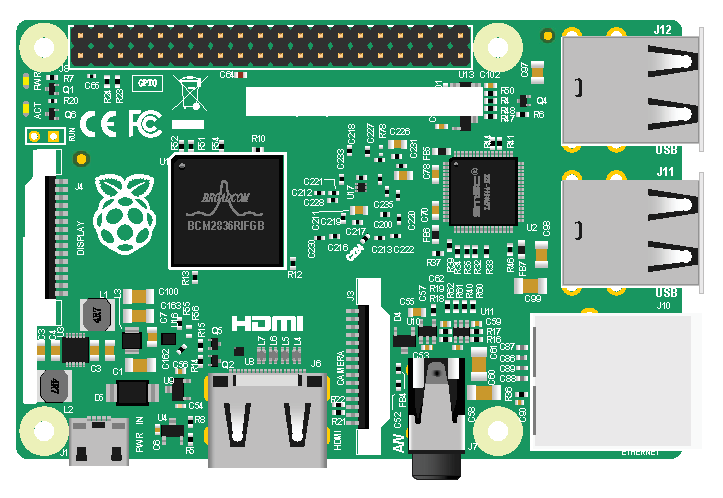
\includegraphics[height=4cm]{figures/rasp.eps}
				\caption{Raspberry Pi板子}
				\label{fig:rasp}
			\end{figure}
		\end{column}
	\end{columns}
	\note{
		Raspberry Pi是一款ARM架构的单板机,
		板载了以太网卡。支持CSI接口,
		方便外接摄像头,进行后期无人机视频传输测试。
		操作系统选择树莓派基金会的Debian系统,
		内核版本为3.18。
	}
\end{frame}
%%Netfilter
\begin{frame}
	\frametitle{Netfilter}
	\begin{columns}
		\begin{column}{0.5\textwidth}
			NC层实施方案有两种:
			\begin{enumerate}
				\item 直接在内核的TCP协议源码上更改,添加NC层的各个模块,然后再编译内核源码
				\item 利用Linux内核提供给用户用于处理网络封包的框架——Netfilter。
			\end{enumerate}
			本文将TCP/NC部署在Netfilter的NF\_IP\_LOCAL\_IN和NF\_IP\_LOCAL\_OUT处。
		\end{column}
		\begin{column}{0.4\textwidth}
			\vspace{-1.5em}
			\begin{figure}
				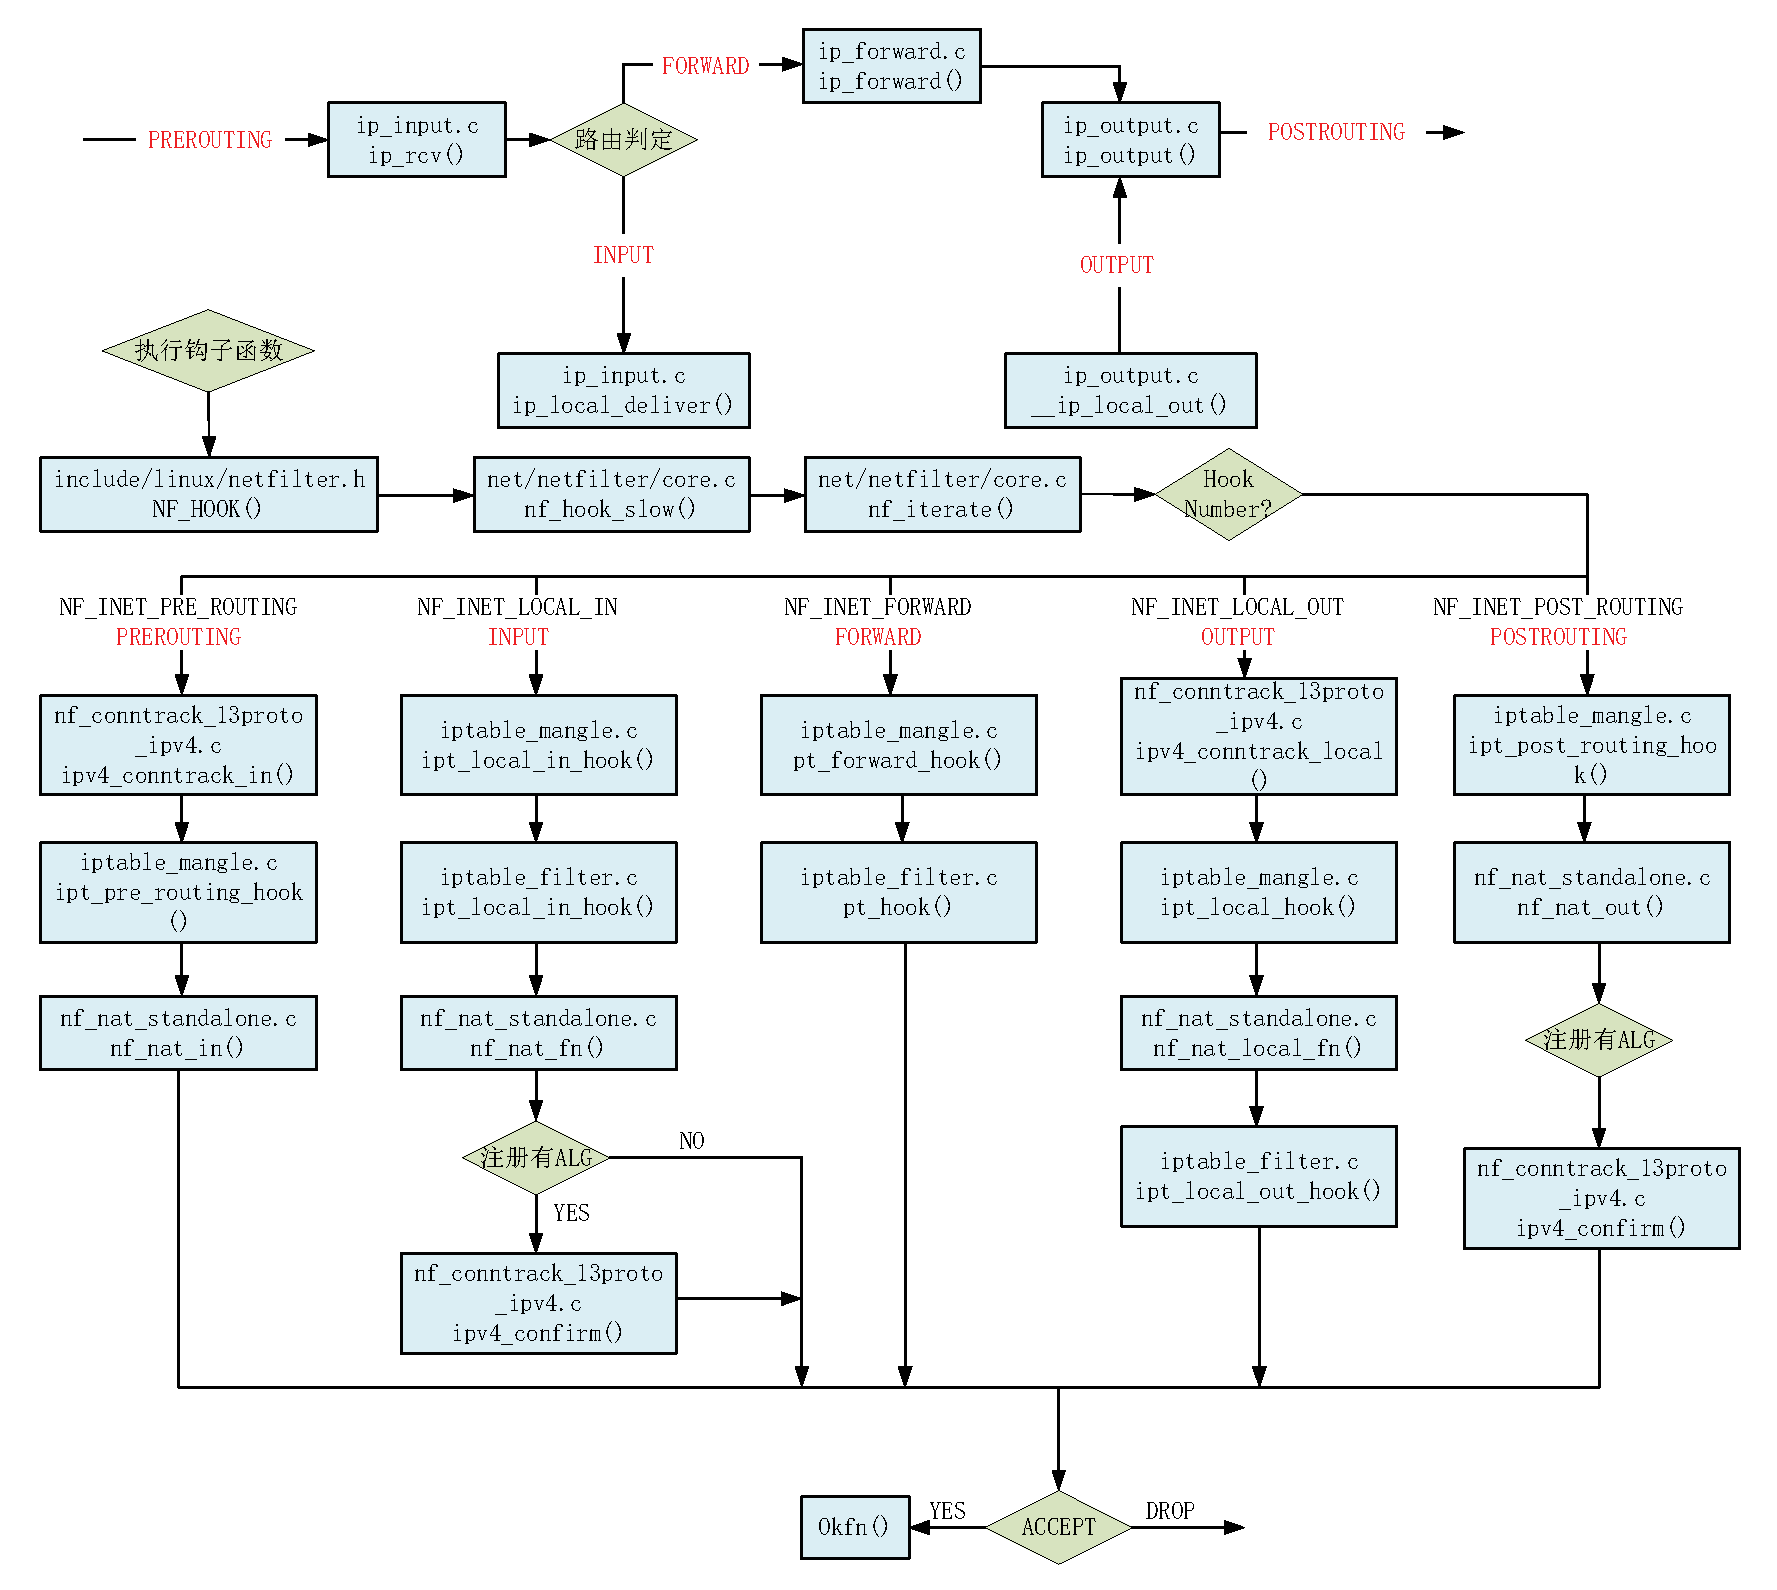
\includegraphics[height=5cm]{../figures/packetflow.eps}
				\caption{Netfilter及其在内核源码中调用关系}
				\label{fig:packetflow}
			\end{figure}
		\end{column}
	\end{columns}

	\note{
	}
\end{frame}
%%关键数据结构
\begin{frame}
	\frametitle{关键数据结构}
	NC层在NF\_IP\_LOCAL\_IN和NF\_IP\_LOCAL\_OUT这两个钩子点获得的都是单独的报文,
	其形式为\emph{sk\_buff}结构体,如图\ref{fig:skbuff}所示。
		\begin{columns}
		\begin{column}{0.5\textwidth}
			数据包在Linux的网络协议栈的不同层之间传递,
			其体现形式就是不同层的函数对一个数据包对应的\emph{sk\_buff}进行各种操作。
			\\
			TCP/NC通过\emph{sk\_buff}获得数据包的字节流,
			然后对数据包进行编码。
		\end{column}
		\begin{column}{0.4\textwidth}
			\vspace{-2em}
			\begin{figure}
				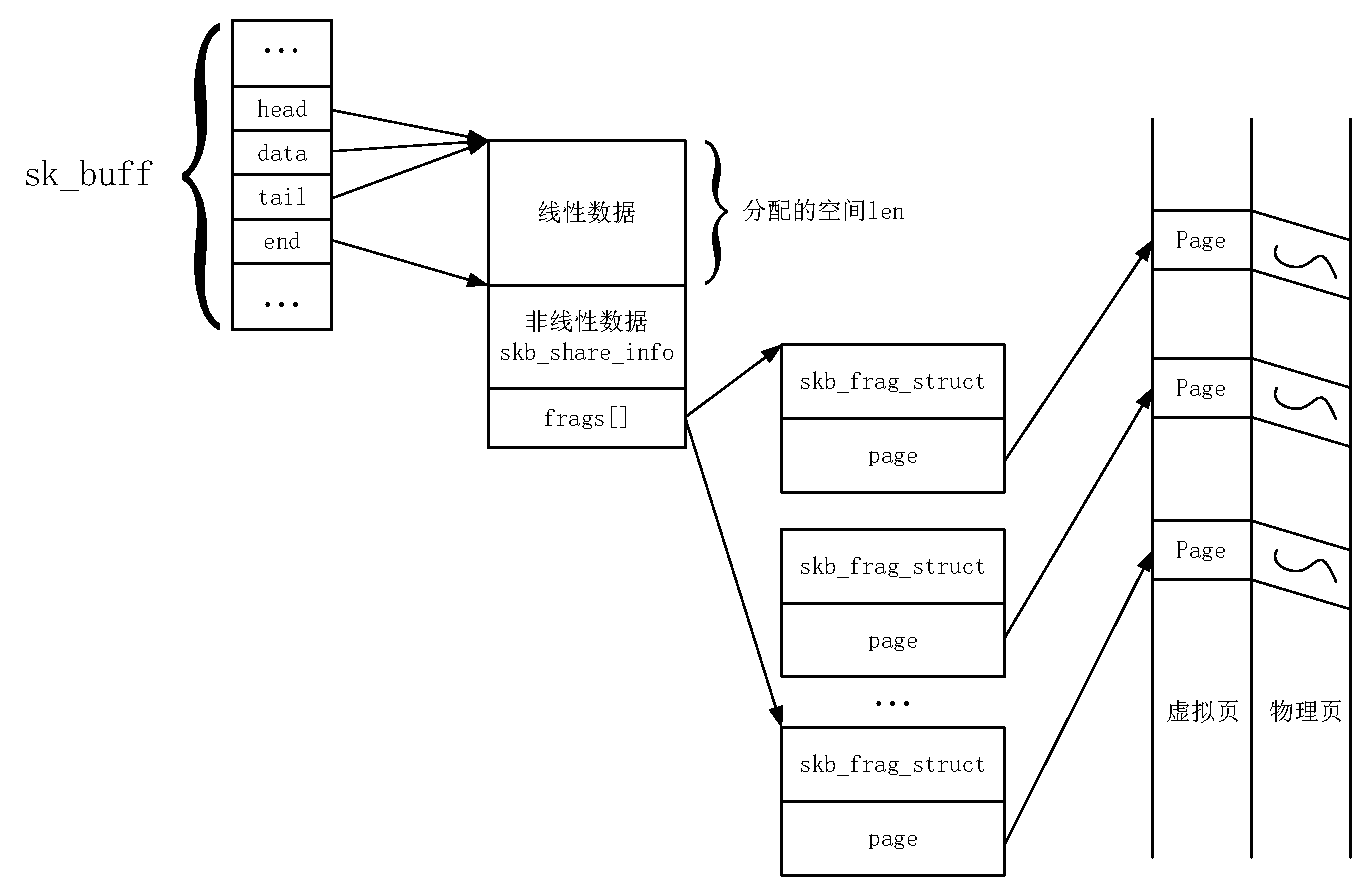
\includegraphics[height=4cm]{../figures/skbuff.eps}
				\caption{skbuff结构}
				\label{fig:skbuff}
			\end{figure}
		\end{column}
	\end{columns}
	
\end{frame}
\subsection{NC层关键技术}

%%NC层总体框架
\begin{frame}[t]
	\frametitle{NC层总体框架}
	\begin{columns}[t]
		\begin{column}{0.4\textwidth}
		图\ref{fig:jiagou}为NC层总体框架。
		虚线框内的即为网络编码层。
		\end{column}
		\begin{column}{0.5\textwidth}
			\vspace{-2.5em}
			\begin{figure}
				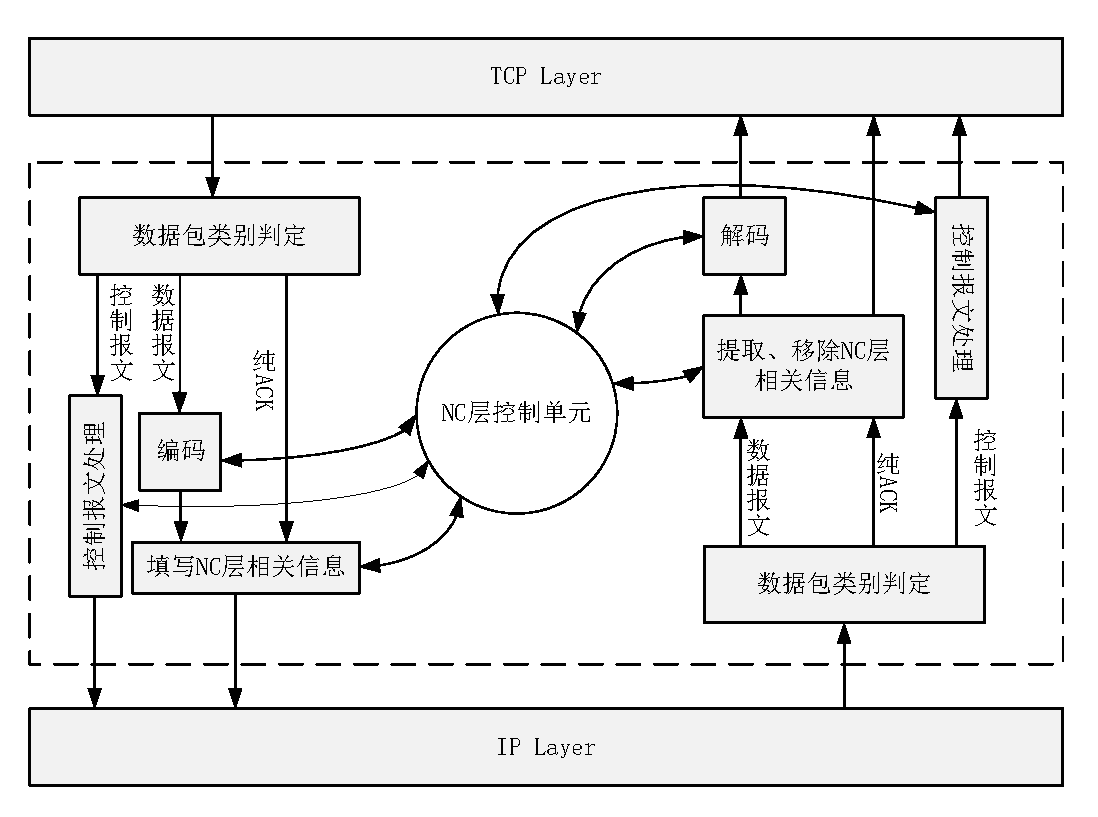
\includegraphics[height=5cm]{../figures/jiagou.eps}
				\caption{NC层总体框架}
				\label{fig:jiagou}
			\end{figure}
		\end{column}
	\end{columns}
\end{frame}
%%NC层头部
\begin{frame}
	\frametitle{NC层头部}
	\begin{columns}
		\begin{column}{0.4\textwidth}
			发送端需要给产生的编码包添加NC头部,
			其中包含编码系数等信息,接收端利用这些信息进行解码。
			图\ref{fig:codingheader}为NC报文的头部。
		\end{column}
		\begin{column}{0.6\textwidth}
			\begin{figure}
				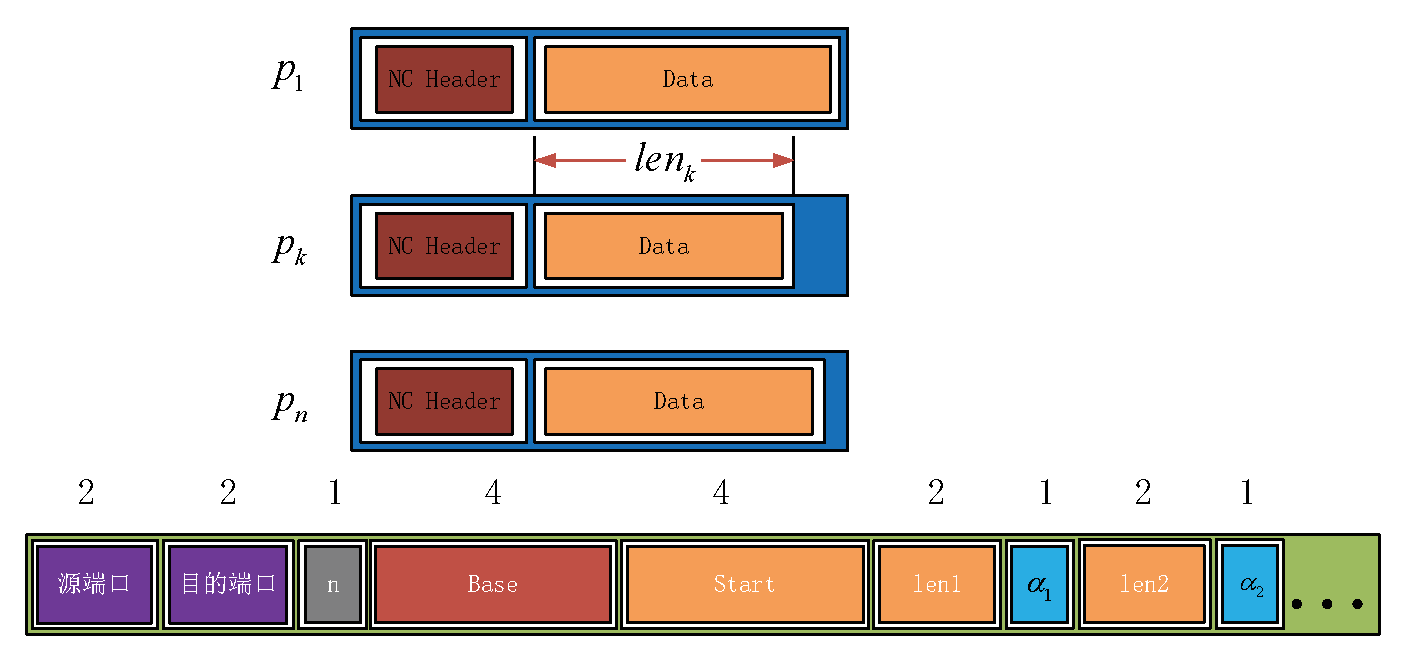
\includegraphics[height=4cm]{../figures/codingheader.eps}
				\caption{NC层头部}
				\label{fig:codingheader}
			\end{figure}
		\end{column}
	\end{columns}
	\note{
	}
\end{frame}
%%编码端
\begin{frame}
	\frametitle{编码}
	\begin{columns}
		\begin{column}{0.4\textwidth}
			发送端的NC层维护了一个\emph{sk\_buff}的链表\emph{sk\_buff\_head},
			存放从TCP层下来的数据包。
			此链表也作为发送端的编码缓存,
			其插入操作发生于有数据包文从TCP层下来时;
			删除操作发生于收到接收端的NC层的ACK报文时。
			编解码步骤如右图。
		\end{column}
		\begin{column}{0.6\textwidth}
			\vspace{-2.5em}
			\begin{figure}
				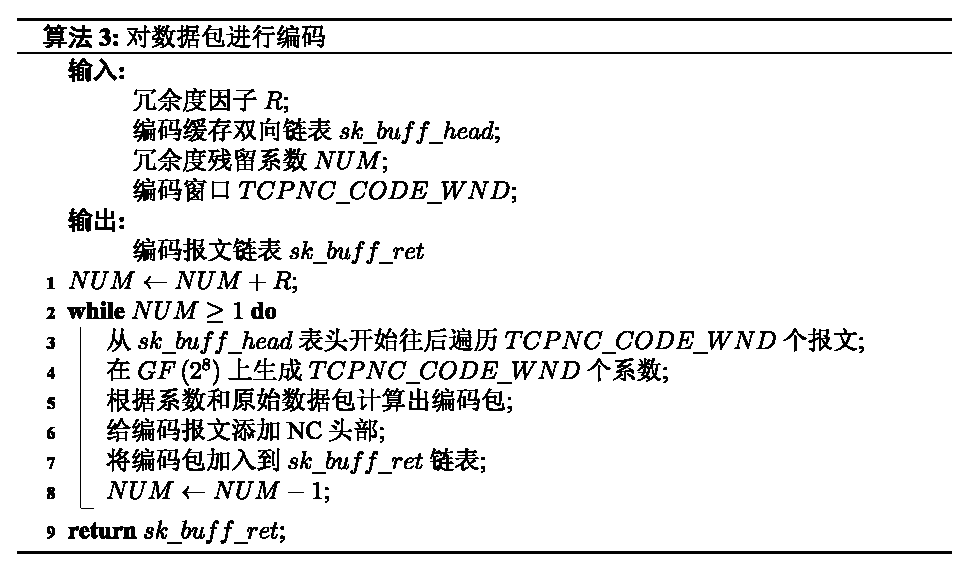
\includegraphics[height=5.5cm]{figures/encoding.eps}
			\end{figure}
		\end{column}
	\end{columns}
\end{frame}

%%解码
\begin{frame}
	\frametitle{解码}
	解码步骤如下:
	\begin{enumerate}
		\item 提取编码报文的编码系数
		\item 对系数进行高斯消元
		\item 利用高斯消元的结果对数据包报文部分进行相应的操作
	\end{enumerate}
	\begin{block}{解码关键技术}
		\begin{enumerate}
			\item \emph{backlog队列},接收端收到的编码数据包首先都会进入\emph{backlog}队列
			\item \emph{decoding队列},\emph{decoding}队列的数据包为目前在解码矩阵中的数据包,可能参与到对数据包的解码操作
			\item \emph{decoded队列},\emph{decoded}队列存放的是目前已经解码出的数据报文。
		\end{enumerate}
	\end{block}
\end{frame}

%%接收窗口
\begin{frame}
	\frametitle{接收窗口}
	考虑到NC层提前确认了一些数据包,
	在接收端,我们需要对发出去的ACK报文的接收窗口值作出修改。
	\begin{figure}
		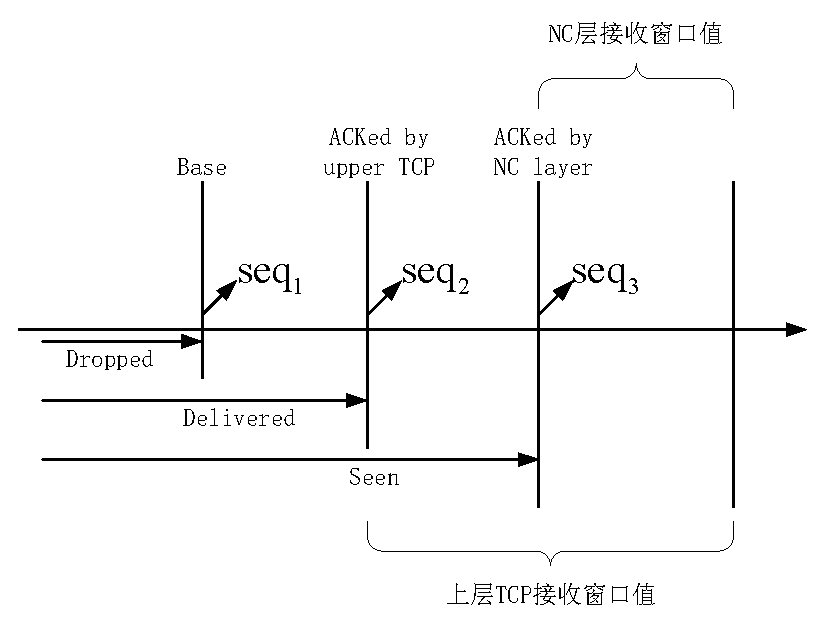
\includegraphics[height=4cm]{../figures/rcvwnd.eps}
		\label{fig:rcvwnd}
		\caption{接收窗口设定}
	\end{figure}
\end{frame}

\subsection{测试结果和结论}
\begin{frame}[allowframebreaks]
	\frametitle{测试}
	\begin{columns}
		\begin{column}{0.4\textwidth}
			\begin{figure}
				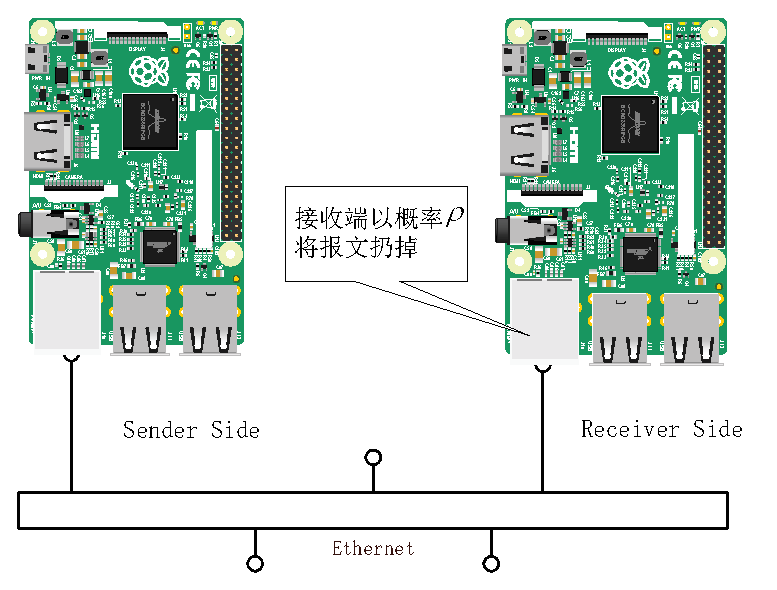
\includegraphics[height=4cm]{../figures/tuopu.eps}
				\label{fig:tuopu}
				\caption{测试拓扑}
			\end{figure}
		\end{column}
		\begin{column}{0.6\textwidth}
			\vspace{-1.5em}
			\begin{table}[htp]
				\centering
				\small
				\caption{测试环境参数}
				\label{tab:ceshicanshu}
				\begin{tabular}{ll}
					\toprule
					参数名称&参数值\tabularnewline
					\midrule
					机型		&Raspberry Pi 2 Model B\tabularnewline
					CPU		&900MHz Cortex-A7\tabularnewline
					RAM			&1G\tabularnewline
					以太网卡 	&10M/100M\tabularnewline
					操作系统 &Debian\tabularnewline
					内核版本 &Linux 3.18\tabularnewline
					TCP协议版本 &TCP-Reno\tabularnewline
					测试工具 &iperf\tabularnewline
					测试时间 &60秒\tabularnewline
					\bottomrule
				\end{tabular}
			\end{table}
		\end{column}
	\end{columns}
	\newpage
	固定链路丢包率为$5\%$,
	测试冗余度对吞吐率的影响如图\ref{fig:throughput2redundancy}。
	
	我们对不同丢包率下TCP和TCP/NC的性能进行了对比测试,
	如图\ref{fig:throughput2loss}所示,
	其中TCP/NC的吞吐率都为最优吞吐率。
	\begin{columns}
		\begin{column}{0.5\textwidth}
			\begin{figure}
				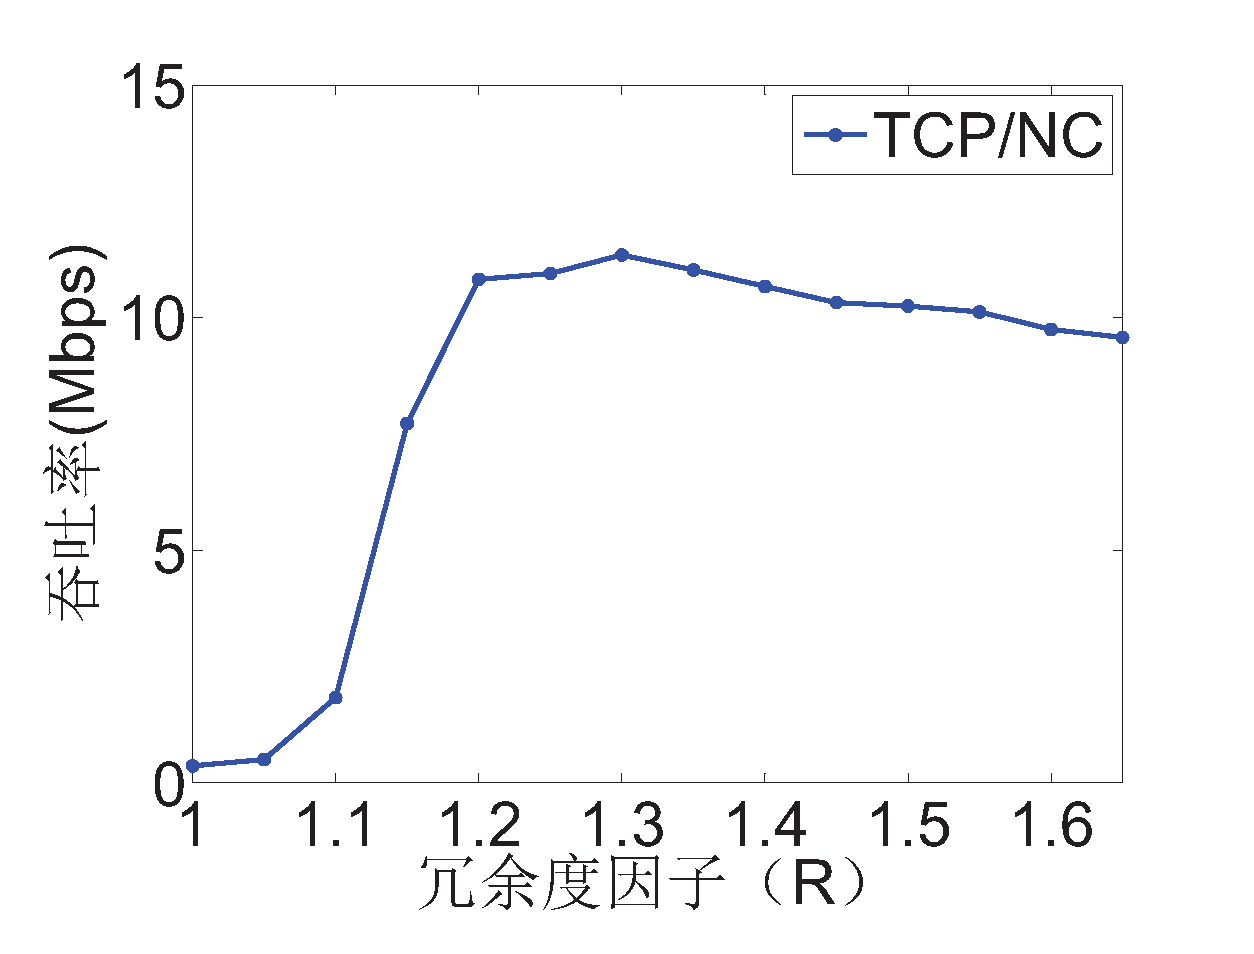
\includegraphics[height=3.5cm]{../figures/redundancy.eps}
				\caption{吞吐率-冗余度}
				\label{fig:throughput2redundancy}
			\end{figure}
		\end{column}
		\begin{column}{0.5\textwidth}
			\begin{figure}
				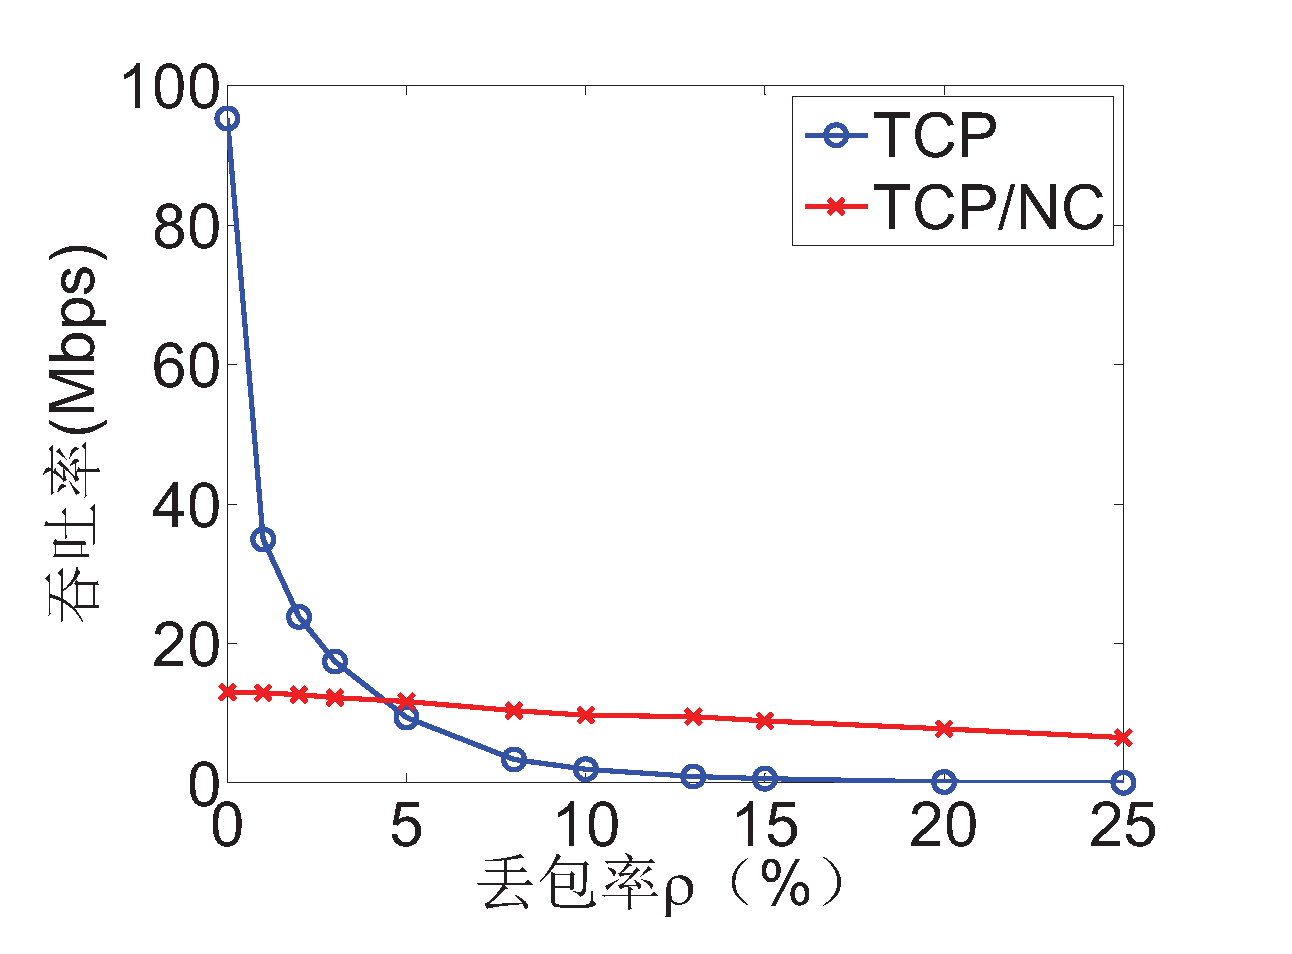
\includegraphics[height=3.5cm]{../figures/throughput2lossrate.eps}
				\caption{吞吐率-丢包率}
				\label{fig:throughput2loss}
			\end{figure}
		\end{column}
	\end{columns}
\end{frame}

%\begin{frame}
%	\frametitle{结论}
%\end{frame}

















%    \section{总结与展望}
%    %添加一个目录
%    \frame{
%     \frametitle{目录}
%     \tableofcontents[current,currentsection,sections={<1-5>}]
%     \addtocounter{framenumber}{-1}  %目录页不计算页码
%    }
%
%    \frame{
%      \frametitle{\secname}
%      \vspace{-0.5em}
%      \begin{block}{总结}
%        \footnotesize
%        \begin{enumerate}[(1)]
%          \item 提出了一种构造紧致凸包围多面体--$k$-CBP~的算法;
%          \item 构造~$k$-CBP~速度上比现有算法快~3$\sim$8~倍;
%          \item 构造的~$k$-CBP~紧致程度比现有的$k$-DOP紧致10\% $\sim$ 40\%;
%          \item 提出了一种基于~$k$-CBP~的碰撞检测算法,该算法较$k$-DOP树算法初始化时间快8倍以上,静止场景快0.8 $\sim$ 3.2 倍,运动场景快0.8 $\sim$ 5.6 倍。
%        \end{enumerate}
%      \end{block}
%      \vspace{-0.5em}
%      \begin{block}{展望}
%        \footnotesize
%      \begin{enumerate}[(1)]
%          \item 碰撞检测算法如何摆脱对AABB树的依赖;应用于近似碰撞检测算法;应用于可变形的模型连续碰撞检测,如何快速更新~$k$-CBP~;
%          \item 如何将~$k$-CBP~应用于如机器人抓取、路径规划等其他应用领域中。
%        \end{enumerate}
%      \end{block}
%      
%      \note{
%        总结一下~\ldots PPT
%      }
%    }

%    \section{主要参考文献}
%    \frame[t,allowframebreaks]{
%      \frametitle{\secname}
%    \printbibliography
%    }
    
    \section{Q\&A}
%    \frame{
%      \frametitle{\secname}
%      \begin{block}{致谢}
%        \begin{enumerate}[(1)]
%          \item 导师雍俊海老师的精心指导;
%          \item 施侃乐老师帮助;
%          \item 研究所各个项目的历练;
%          \item 王斌老师、陈莉老师的评审及意见,答辩委员会老师聆听和指导。
%        \end{enumerate}
%      \end{block}
%    }
    \frame{
      \frametitle{Q \& A}
      \begin{block}{Questions?}
       ~\\ ~\\
       \center{\Large{Thank you!}}
       \\ ~\\ ~\\ ~\\ ~\\ 
      \end{block}
    }



%    \section{总结与展望}
%    %添加一个目录
%    \frame{
%     \frametitle{目录}
%     \tableofcontents[current,currentsection,sections={<1-5>}]
%     \addtocounter{framenumber}{-1}  %目录页不计算页码
%    }
%
%    \frame{
%      \frametitle{\secname}
%      \vspace{-0.5em}
%      \begin{block}{总结}
%        \footnotesize
%        \begin{enumerate}[(1)]
%          \item 提出了一种构造紧致凸包围多面体--$k$-CBP~的算法;
%          \item 构造~$k$-CBP~速度上比现有算法快~3$\sim$8~倍;
%          \item 构造的~$k$-CBP~紧致程度比现有的$k$-DOP紧致10\% $\sim$ 40\%;
%          \item 提出了一种基于~$k$-CBP~的碰撞检测算法,该算法较$k$-DOP树算法初始化时间快8倍以上,静止场景快0.8 $\sim$ 3.2 倍,运动场景快0.8 $\sim$ 5.6 倍。
%        \end{enumerate}
%      \end{block}
%      \vspace{-0.5em}
%      \begin{block}{展望}
%        \footnotesize
%      \begin{enumerate}[(1)]
%          \item 碰撞检测算法如何摆脱对AABB树的依赖;应用于近似碰撞检测算法;应用于可变形的模型连续碰撞检测,如何快速更新~$k$-CBP~;
%          \item 如何将~$k$-CBP~应用于如机器人抓取、路径规划等其他应用领域中。
%        \end{enumerate}
%      \end{block}
%      
%      \note{
%        总结一下~\ldots PPT
%      }
%    }


\section{主要参考文献}
\frame[t,allowframebreaks]{
	\frametitle{\secname}
	\printbibliography
}
    
\section{Q\&A}
    \frame{
%      \frametitle{\secname}
      \begin{block}{致谢}
        \begin{enumerate}[(1)]
          \item 导师陈庆春老师的精心指导;
          \item 教研室各位同学三年来对我的帮助;
          \item 教研室各个项目的历练;
          \item XX老师、XX老师的评审及意见,答辩委员会老师聆听和指导。
        \end{enumerate}
      \end{block}
    }
    \frame{
      \frametitle{Q \& A}
      \begin{block}{Questions?}
       ~\\ ~\\
       \center{\Large{\emph{Thank you!}}}
       \\ ~\\ ~\\ ~\\ ~\\ 
      \end{block}
    }


\end{document}

